%% bare_jrnl.tex
%% V1.4
%% 2012/12/27
%% by Michael Shell
%% see http://www.michaelshell.org/
%% for current contact information.
%%
%% This is a skeleton file demonstrating the use of IEEEtran.cls
%% (requires IEEEtran.cls version 1.8 or later) with an IEEE journal paper.
%%
%% Support sites:
%% http://www.michaelshell.org/tex/ieeetran/
%% http://www.ctan.org/tex-archive/macros/latex/contrib/IEEEtran/
%% and
%% http://www.ieee.org/

\documentclass[journal]{IEEEtran}
%
% If IEEEtran.cls has not been installed into the LaTeX system files,
% manually specify the path to it like:
% \documentclass[journal]{../sty/IEEEtran}

\usepackage[cmex10]{amsmath}
\usepackage{graphicx}
\usepackage{mathtools}
\usepackage{subfigure}
\usepackage{epstopdf}
\usepackage{enumitem}
\usepackage{cite}
\usepackage{hhline}
\usepackage{color,soul}

\DeclarePairedDelimiter{\abs}{\lvert}{\rvert}

% correct bad hyphenation here
\hyphenation{op-tical net-works semi-conduc-tor}


\begin{document}
%
% paper title
% can use linebreaks \\ within to get better formatting as desired
% Do not put math or special symbols in the title.
\title{Multiple Dice Working as One: CAD Flows and Routing Architectures for Silicon Interposer FPGAs}
%
%
% author names and IEEE memberships
% note positions of commas and nonbreaking spaces ( ~ ) LaTeX will not break
% a structure at a ~ so this keeps an author's name from being broken across
% two lines.
% use \thanks{} to gain access to the first footnote area
% a separate \thanks must be used for each paragraph as LaTeX2e's \thanks
% was not built to handle multiple paragraphs
%

\author{
		% 1st author
		Ehsan~Nasiri,
		% 2nd author
		Javeed~Shaikh,
		% 3rd author
		Andre~Hahn~Pereira,
		% 4th author
        and~Vaughn~Betz,~\IEEEmembership{Member,~IEEE}%
\thanks{E. Nasiri is with Altera, Toronto, ON, Canada (email: enasiri@altera.com)}% 
\thanks{J. Shaikh is with Google, Mountain View, CA, USA (email: jvds@google.com)}%
\thanks{A. H. Pereira is with the Computer and Digital Systems Engineering Dept., University of S\~{a}o Paulo, SP, Brazil (email: andre.hahn@usp.br)}%
\thanks{V. Betz is with the Dept. of Electrical and Computer Engineering, University of Toronto, ON, Canada (email: vaughn@eecg.utoronto.ca)}%
\thanks{Manuscript received January 6, 2015.}}


% make the title area
\maketitle

% As a general rule, do not put math, special symbols or citations in the abstract or keywords.
\begin{abstract}
Large FPGA systems with multiple dice connected by a silicon interposer are now commercially available. However, many questions remain concerning their key architecture parameters and efficiency, as the signal count between dice is reduced and the delay between dice is increased compared to a monolithic FPGA. We modify VPR to target interposer-based FPGAs and investigate placement and routing changes and incorporating partitioning into the flow to improve results. Our best CAD flow reduces the routing demand for interposer FPGAs with realistic connectivity between dice by 47\% and improves the circuit speed by 13\% on average. Architecture modifications to add routing flexibility when crossing the interposer are very beneficial and improve routability by a further 11\%. With these CAD and architecture enhancements, we find that if an interposer supplies (between dice) 20\% of the routing capacity that the normal (within-die) FPGA routing channels supply, there is only a modest impact on circuit routability. Smaller interposer routing capacities do impact routability however: minimum channel width increases by 70\% when an interposer supplies only 10\% of the within-die routing. The interposer also impacts delay, increasing circuit delay by 11\% on average for a 1 ns interposer signal delay and a two-die system.
\end{abstract}

% Note that keywords are not normally used for peerreview papers.
\begin{IEEEkeywords}
FPGA, Silicon interposer, 2.5D ICs, CAD. 
\end{IEEEkeywords}



\section{Introduction}
\label{introSection} 
%   - Describe multi-chip
Interposer-based FPGA systems are composed of multiple FPGA dice connected through a silicon interposer. The interposer uses an older fabrication technology than the FPGA dice, and links between dice include both a micro-bump on each FPGA die and a metal wire on the interposer~\cite{xilinxTSVperformance}. This results in reduced connectivity and increased delay between dice compared to the routing bandwidth and delay across a cutline within a single die. Such interposer systems are sometimes called 2.5D devices, since they make use of vertical stacking of dice on an interposer to enable higher integration levels~\cite{3dhandbook}. In this work we present an architecture study of silicon interposer-based FPGAs that analyzes how the reduced connectivity and increased delay impact their performance.

Silicon interposers enable the creation of large FPGAs from smaller dice, which can both improve yield and fabricate FPGAs that are too large to be manufacturable on a single die. Making large FPGAs from multiple smaller dice is particularly interesting at the beginning of a new manufacturing process, when defect densities are high. In this case, good-die yield drops dramatically as the die size increases, drastically impacting the availability of large FPGAs early in the process lifetime.

%   - Prior work (El Gamal, Xilinx WP, Xilinx paper) - TODO
The idea of using 3 dimensions to design FPGAs is not new. \hl{Alexander et al} \cite{3dfpga1995} proposed the creation of 3D FPGAs by stacking 2D FPGAs and connecting them with solder bumps. Lin et al also studied 3D FPGAs, but using a different approach~\cite{3dfpga} that utilized multiple active layers with different FPGA functions (logic, routing, and configuration) in each. While promising, both these approaches have manufacturing challenges: \cite{3dfpga1995} requires a higher density of through-silicon vias than can currently be manufactured and the multiple active layers required by \cite{3dfpga} are not yet widely available. In contrast, silicon interposers linked to dice via microbumps are now manufacturable.

Chaware et al presented Xilinx's approach to silicon interposer FPGAs~\cite{xilinxTSV}. They describe the physical characteristics of their implementation, including the bump pitch and estimates of the amount of die-to-die connectivity and the die-to-die delay. However~\cite{xilinxTSV} does not analyze the architecture question of the routability of the resulting system, nor describe possible CAD optimizations, which are the questions we investigate.

%   - Contributions
The main contributions of our work are as follows:
\begin{itemize}
	\item VPR CAD tool modifications to model and optimize for 2.5D silicon interposer-based FPGAs.
	\item An investigation of the efficacy of incorporating partitioning into various stages of the CAD flow.
	\item A study of how multi-FPGA system routability is impacted by the amount of between-die connectivity and by the switching flexibility at the FPGA die - interposer boundary.
	\item An analysis of the interposer's impact on timing.
\end{itemize}

The paper is organized as follows. Section \ref{siliconSection} gives more information about silicon interposer technology. Section \ref{archSection} describes the changes made to the FPGA architecture description and VPR to target 2.5D FPGAs. Section \ref{cadSection} describes optimizations to the VPR placement and routing algorithms for interposer FPGAs and Section~\ref{sec:CADflow} describes how partitioning can further enhance the CAD flow. Section \ref{resultsSection} presents architectural results for 2.5D FPGAs.

An earlier and less detailed version of this work appeared in \cite{interposer2014}. We greatly extend this earlier work by enhancing the CAD tools, incorporating partitioning into the flows and investigating a broader range of architecture questions. 


\section{Silicon Interposer Background}
\label{siliconSection}

Interposer-based FPGAs allow systems larger than a single die, making a "More than Moore" improvement \cite{arden2010morethan} on the size and number of logic cells possible, and with chips combined with far more connectivity and less delay than if they were in separate packages connected through a printed circuit board. 

The improvement in the capacity of 2.5D FPGAs over conventional ones is very significant. Xilinx's largest 28 nm interposer-based FPGA contains 4 FPGA dice and 1.954 million logic cells~\cite{xilinx7series}, while the largest non-interposer Virtex-7 die has 979k logic cells and Altera's largest 28 nm FPGA has 952k logic elements~\cite{stratixV}. Even though all these FPGAs use a 28 nm process, silicon interposer technology allows the creation of FPGAs with twice the resources possible on even an extremely large single die. Xilinx's latest (Virtex UltraScale, 20 nm) line of FPGAs makes even more aggressive use of interposers; the largest monolithic FPGA in this family contains 941k logic cells, while the four largest capacity FPGAs are all built with silicon interposers and span a range from 1.25 to 4.43 million logic cells~\cite{virtexultrascale}.

Another major advantage of interposer-based FPGAs comes at the beginning of a new manufacturing process, when the defect density is high~\cite{xilinxTSVperformance}. To illustrate this impact consider a new process in which the defect density is 1/$cm^2$ and the die area is $6cm^2$, roughly matching the size of the largest member of a high-end FPGA family such as Virtex 7. Using the Poisson Yield Model~\cite{yieldmodel}, the yield is only $0.25\%$ of dice. If instead the chip is composed of four $1.5cm^2$ dice, the yield is $22\%$. This means that a 12 inch silicon wafer with $730cm^2$ of area would produce on average $0.3$ working $6cm^2$ dice, while the same wafer would produce on average $107$ working $1.5cm^2$ dice. Therefore, as a $6cm^2$ chip would be composed of four $1.5cm^2$ dice, the wafer would yield $26.75$ systems on average, as the "assembly yield" of placing these four die on an interposer is very high~\cite{xilinxTSV}. Hence the number of interposer-based FPGAs created from the same silicon wafer would be almost $100\times$ greater than a monolithic FPGA of the same size, greatly impacting not only cost but also the availability of such a large FPGA.

When the process matures and the defect density decreases this yield advantage drops. Consider a mature process with defect density of $0.1/cm^2$. The yield for a $6cm^2$ die is $55\%$ and the yield for a $1.5cm^2$ die is $86\%$. Hence the number of single die FPGAs created from a $730cm^2$ silicon wafer would be $66.9$ and the number of interposer-based FPGAs created would be $104.6$. While the interposer-based FPGA still has a yield advantage it might not lead to a major cost advantage when the cost of the interposer and die assembly costs are included. For the large, state-of-the-art FPGAs that are built early in a process cycle and heavily used for prototyping, however, there is clearly a compelling cost advantage to an interposer-based solution.

\subsection{Virtex Interposer-based FPGAs}
\label{virtex7section}

The Xilinx 2.5D FPGAs from the Virtex-7 and Virtex Ultrascale families are currently the only commercially available silicon interposer-based FPGAs~\cite{xilinxWP}. \hl{We are studying} the impact of several key interposer parameters on the performance of the multi-die system, including (i) the percentage of the wiring normally present between rows of the FPGA which is cut when crossing between dice, and (ii) the extra delay (vs. a normal connection between adjacent rows) added when one must traverse the interposer.  To locate where Virtex-7 lies in this architecture space, we combined published information on the implementation of Xilinx's interposer-based FPGAs~\cite{xilinxTSV} with a detailed analysis of the~\textit{XC7V2000T} FPGA routing resources visible in the \textit{Vivado Device View}.

\begin{figure}[!htbp]
\centering
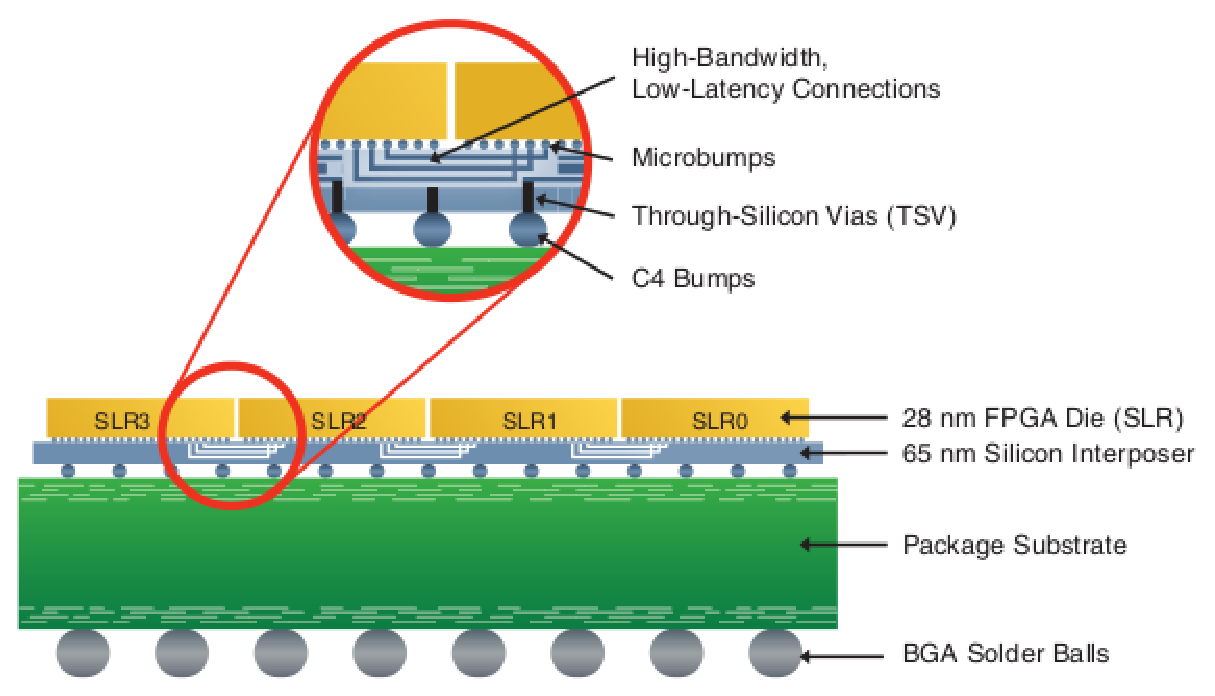
\includegraphics[width=\linewidth]{interposer.eps}
\caption{Lateral view of an interposer-based FPGA\cite{xilinxWP}. The FPGA dice are at the top, and are connected to the silicon interposer through microbumps. The interposer is then connected to the substrate through C4 bumps.}
\label{fig:interposer}
\end{figure}

% Xilinx details:
%  -> 13440 wires crossing
%  -> ~63k vertical wires
%  -> Micro-bumps -> pitch is 45um
%  -> Spread out near edge, to get more bumps
%  -> But results in longer signal travel
%  -> Net result: more delay, reduced connectivity

The \textit{XC7V2000T} is composed of four identical dice arranged such that the vertical routing crosses between the dice. Each horizontal edge of each die has 280 groups of 48 length-12 wires crossing the interposer, for a total of 13440 wires between dice. There are also 40 clock wires crossing the interposer. The average vertical routing channel in this FPGA contains 210 wires and there are approximately 280 vertical channels, resulting in approximately 58800 vertical wires crossing a horizontal cutline within a die. Hence the number of wires which cross the interposer is about 23\% of the total number of within-die vertical wires.

The 28 nm dice are connected to the 65 nm silicon interposer through microbumps with a 45$\mu$m pitch. Hence the area occupied by microbumps at one edge of one die is 13440 $\times$ (45$\mu$m)\textsuperscript{2} $=$ 27mm\textsuperscript{2}. If we assume each die is $7 \times 12 mm$, as presented by Chaware et al. in \cite{xilinxTSV}, the bumps have to be spread out near the edge and need to go as far as $2.25mm$ away from the edge of the die. This greater distance from the border increases the length of the inter-die connections, and along with the presence of the micro-bumps and their capacitance, leads to an increased delay for these crossing wires vs. that of a typical on-die routing wire. Chaware et al. state that the latency to cross the interposer is approximately $1ns$. For comparison, a typical medium length 28 nm FPGA routing wire (e.g. spanning four logic blocks) has a delay of approximately 125 ps, while a longer wire (e.g. spanning 12 logic blocks) has a delay of approximately 250 ps.

Overall, these interposer FPGAs have increased delay and reduced connectivity between dice, with approximately $23\%$ of the usual number of vertical wires between dice and approximately $1ns$ of increased delay to cross the interposer.

%---------------------------------------------------------------
%---------------------------------------------------------------
%---------------------------------------------------------------
\section{Architecture Models}
\label{archSection}
%   - Define parameters
To properly model a silicon interposer FPGA, we use version 7.0 of the popular FPGA exploration toolset, Verilog-to-Routing (VTR)~\cite{luu2014vtr}. The logic synthesis portions of the flow (ODIN II and  ABC) are used as-is, while we modify the placement and routing portion of the flow (VPR~\cite{betz1997vpr}) to model and optimize for interposer-based FPGAs. The modifications are made in such a way that they require no changes to any of the input files, so one can experiment with interposer-based FPGAs with any existing benchmark circuits and any existing VPR-format FPGA architecture description simply by specifying appropriate command-line parameters.

We add the following parameters to VPR: \textit{number of cuts}, \textit{\% wires cut}, \textit{increased delay}, and \textit{interposer-routing interface}. These parameters describe the interposer portion of the 2.5D FPGA as detailed below.

%	- number of cuts
\subsection{Number of Cuts}
\textit{Number of cuts} describes how many cuts are made to the interposer-based FPGA versus a monolithic die. If \textit{number of cuts} equals 1 then there are 2 dice, and so on. We investigate values of 1 and 3 (2 and 4 dice). The Virtex 7 family has members with \textit{number of cuts} $=$ 2 and 3. Figure \ref{fig:fpga} shows a sample architecture with one cutline.

\begin{figure}[!htbp]
\centering
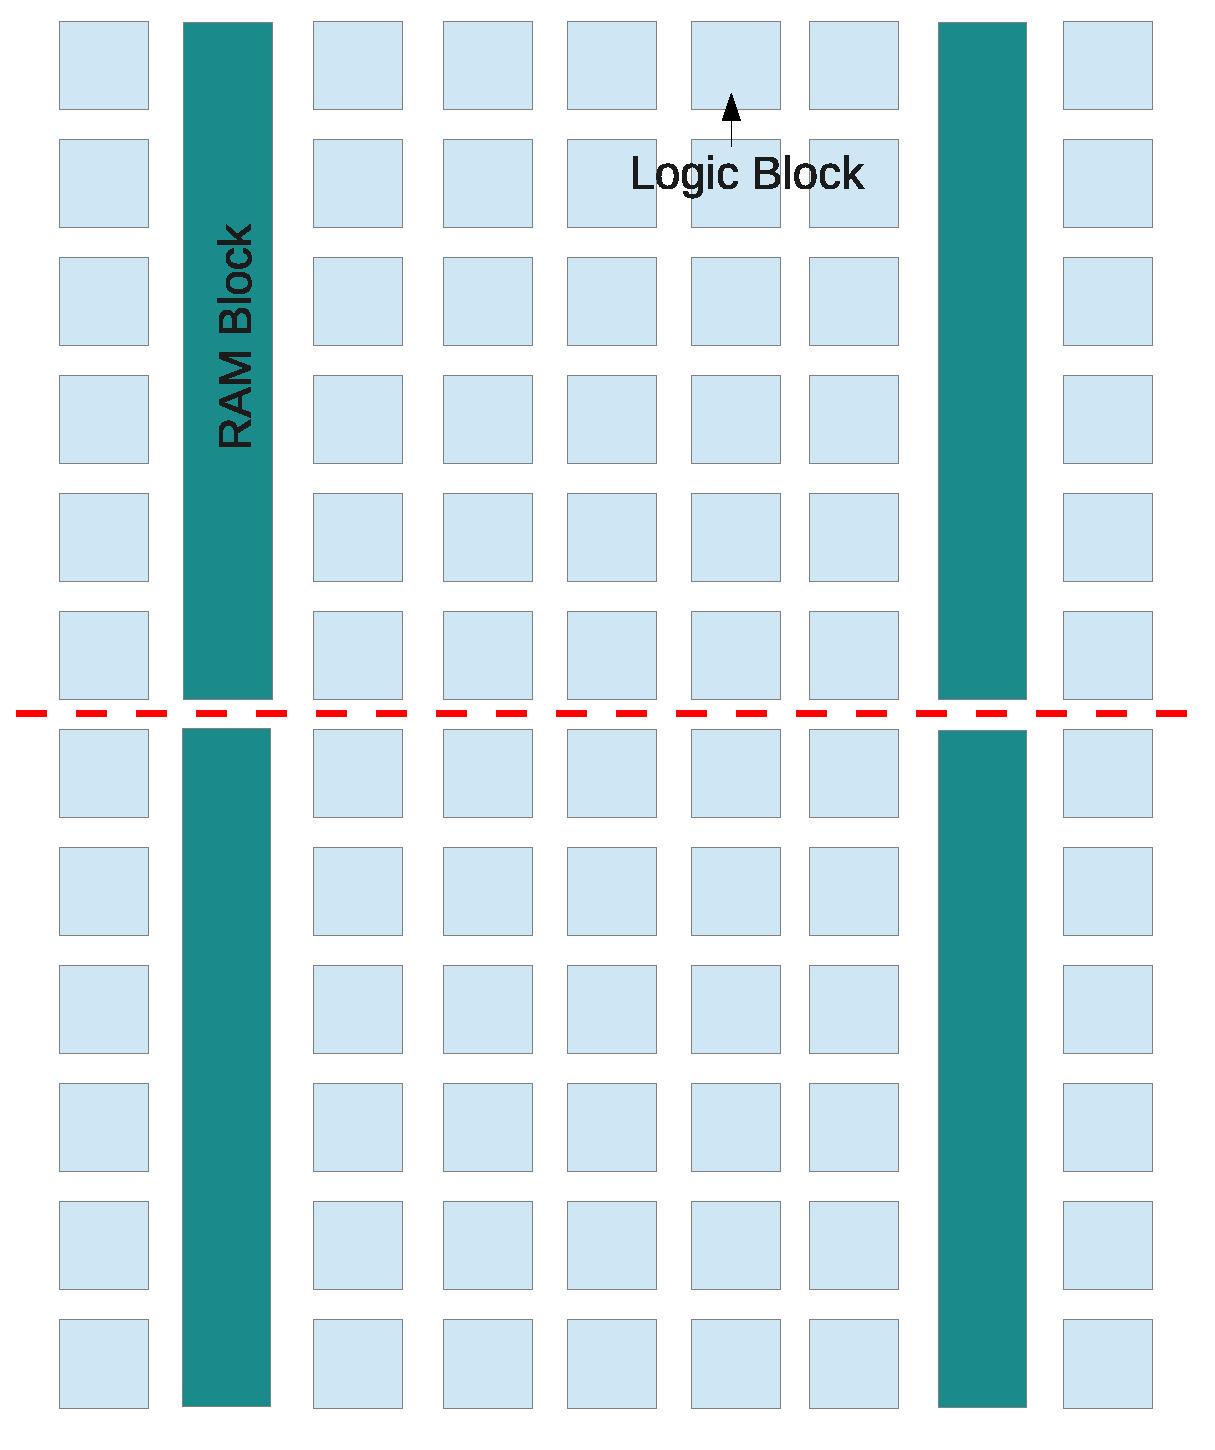
\includegraphics[width=0.6\linewidth]{fpga.eps}
\caption{A sample two-die / 1-cutline architecture containing both logic blocks and RAM blocks.}
\label{fig:fpga}
\end{figure}

%   - % wires cut
\subsection{\% Wires Cut}
This variable describes and models the reduced connectivity between different dice by specifying the fraction of routing wires that are removed at the border between dice. For example, if a channel had 200 wires and \textit{\% wires cut} was 70, 140 of them would be cut and only 60 would pass through the interposer. Higher values of \textit{\% wires cut} make an interposer easier to manufacture, and can reduce the interposer delay by allowing all the microbumps linking dice to be placed near the die edge. However, the higher \textit{\% wires cut} is, the less routable the multi-die system becomes. As described in \ref{virtex7section}, the Virtex 7 family has \textit{\% wires cut} $=$ 77\%.

%   - Added delay
\subsection{Increased Delay}
Interposer wires are longer and wider than on-die wires and have microbumps on each end. \textit{Increased delay} models the resulting larger delay when compared with wires which are internal to a die. A reasonable estimate for this variable is around $1ns$, as presented by Chaware et al\cite{xilinxTSV}.

%   - Interposer-Routing interface
\subsection{Interposer-Routing Interface}
\label{sec:interposer-routing-interface}
In a simple architecture, the vertical routing wires at the edge of an FPGA die that can not connect to an interposer wire are dangling. Since interposer wires are scarce, we want to be able to study architectures in which the interposer wires are more accessible. To do so, we have enhanced the router to support the following interposer-routing interface options.

\begin{enumerate}
\item Fan-in Transfer for Interposer Wires\\
For an architecture with \textit{\% wires cut} $=0$, all vertical routing wires have a corresponding interposer wire that connects them to the adjacent die. Practical interposers, however, can only accommodate a fraction of all vertical routing wires. \hl{As shown in Figure}~\ref{fig:architecture_params}, when \textit{fanin transfer} option is \textit{on}, we place a multiplexer at the input of each available interposer wire and connect adjacent ``dangling" vertical routing wires to the multiplexer. This enables additional flexibility in routing by ensuring that \textit{every} vertical routing wire could \textit{potentially} drive an interposer wire through a multiplexer. As an example, if \textit{\% wires cut} $=75\%$, 3 of every 4 interposer wires are cut. Therefore, we place a 4-to-1 mux at the input of the one interposer wire that is not cut, and we connect the 3 vertical routing wires that do not have a corresponding interposer wire to the multiplexer. 

\item Fan-out Transfer for Interposer Wires\\
\hl{As shown in Figure}~\ref{fig:architecture_params}, when \textit{fanout transfer} option is \textit{on}, we allow an interposer wire to drive not only its own corresponding vertical wire at the other side of the cut, but also other ``dangling" vertical routing wires that are not driven by anything because their corresponding interposer wires are cut.

\item Bidirectional Interposer Wires\\
Dominant routing architectures in modern FPGAs use unidirectional wires~\cite{unidirectional, lewis2005stratix} which can only be driven at one point, normally their start point. When this option is \textit{on}, we allow interposer wires to be driven from one end or the other by adding tri-state buffers at both ends.
\end{enumerate}

\begin{figure}[!htbp]
\centering
\includegraphics[width=0.75\linewidth]{architecture_params.eps}
\caption{For a channel width of 4 and 75\% wires cut, only 1 interposer wire exists (in green) and 3 interposer wires are cut (in the red). (a)~Fan-in Transfer for Interposer Wires allows red routing wires in die 1  to drive a mux that allows them to cross the interposer layer. (b)~Fan-out Transfer for Interposer Wires allows the output of the interposer wire to drive wires in other tracks in die 2.}
\label{fig:architecture_params}
\end{figure}

These options are independent and can be combined to achieve more flexible routing. Enabling any of these options requires adding specific circuitry (such as multiplexers) on the dice which causes very small area and delay increase that we neglect in our experiments.

%   - (briefly) explain how it was put in VPR
\subsection{Implementation}
To model an interposer-based multi-FPGA system in the CAD tool, we use the existing VPR infrastructure for monolithic FPGAs and make several modifications to it.

First, the presence of multiple dice in an interposer-based FPGA is modeled by creating horizontal cuts in the FPGA. The \textit{number of cuts} is specified by the user, and we use that to determine the y-location of the cuts. The cutlines ``snap to the grid" such that the height of all dice are equal and no cutline cuts through a block. For instance, a RAM block of height 4 must remain a unit and can not be sliced by a cutline.

Second, knowing the location of the cutlines, the placer uses the \textit{(x,y)} coordinate of any pin or block to determine the die to which it belongs. The placer uses this information as well as \textit{interposer delay} to better decide where to place each netlist block in order to minimize the cost of inter-die signal transfer as described in Section \ref{cad_enh_placer_subsection}.

Third, the Routing Resource Graph (\textit{rrgraph}) must be modified. The rrgraph is the data structure that defines all the available routing wires (\textit{rrnodes}) and switches in the FPGA, as well as the delay of each~\cite{betz1999architecture}. Given a suitable rrgraph, the VPR router can implement circuits in the desired FPGA, and the VPR timing analyzer can estimate their delay. In the experiments below, we use an architecture that has only unidirectional wires.

Previous work by Pereira et al \cite{interposer2014} modeled the interposer indirectly: they did not introduce new rrnodes in the rrgraph to represent the interposer wires. Rather, they found the rrnodes that cross a cutline. Then they either removed all outgoing edges of these rrnodes (if the routing node was part of the \textit{\% wires cut}), or, they increased the switch delay of the rrnode fan-outs (if the wire was not cut) to account for the additional interposer delay.

While this is a reasonable method to model such architectures, it makes it difficult to experiment with different routing-interposer interfaces such as placing input muxes for interposer wires. Therefore, we modify the rrgraph differently to more accurately reflect the interposer layer directly.

\begin{figure}[!t]
\subfigure[]{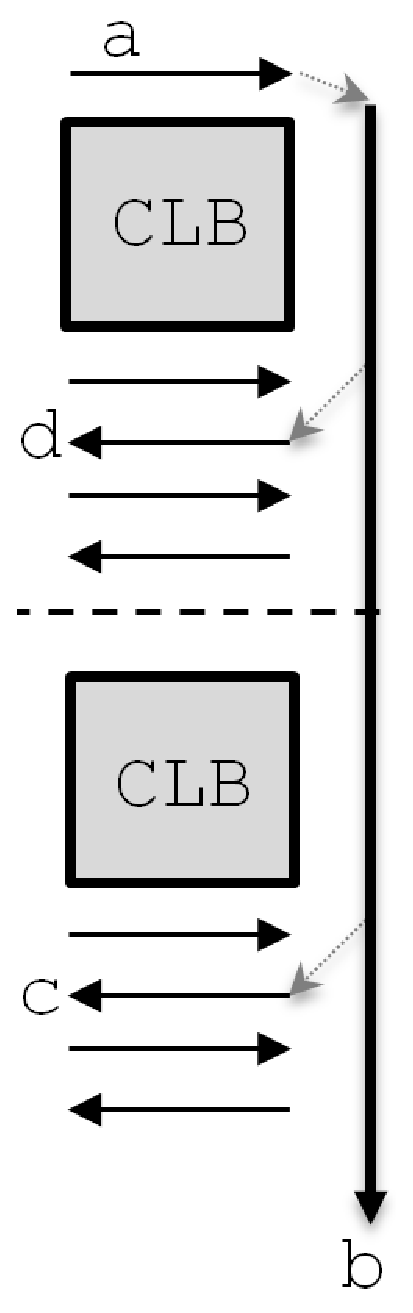
\includegraphics[width=0.17\linewidth]{a.eps}}
\subfigure[]{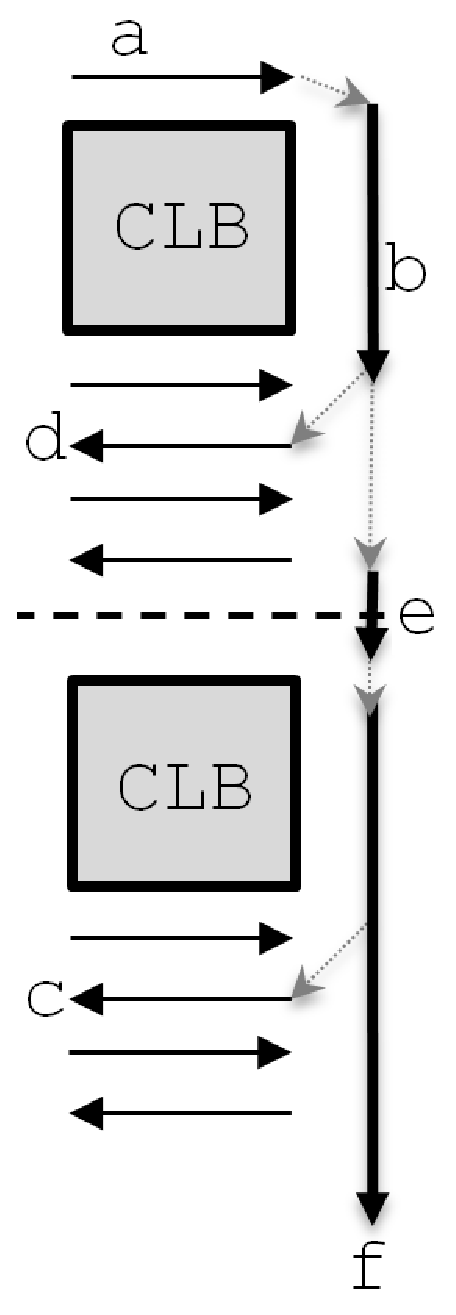
\includegraphics[width=0.17\linewidth]{b.eps}}
\subfigure[]{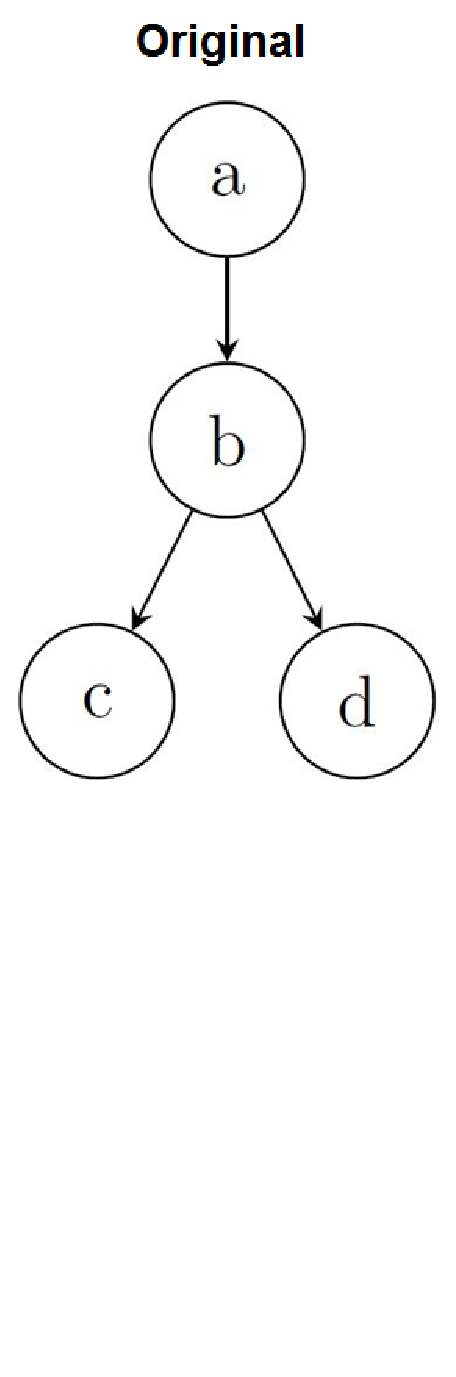
\includegraphics[width=0.17\linewidth]{a_prime.eps}}
\subfigure[]{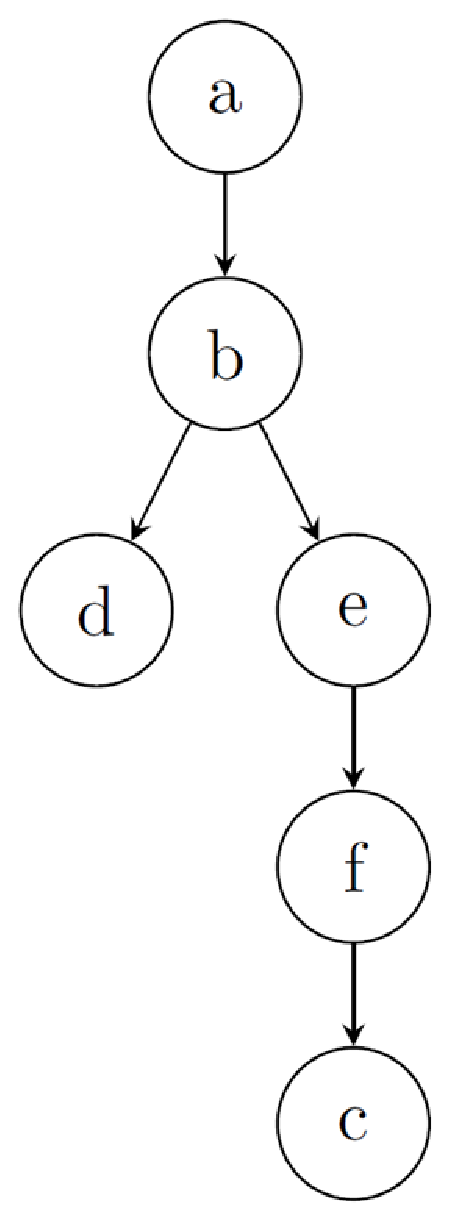
\includegraphics[width=0.17\linewidth]{b_prime.eps}}
\caption{(a) Regular routing wire connectivity. (b) Replacing the long wire with two wires and connecting them via an interposer wire. (c) rrgraph for regular connectivity. (d) rrgraph after modifications.}
\label{fig:rrgraph_ops}
\end{figure}

\begin{figure*}[!thpb]
\centering
\subfigure[]{\includegraphics[width=0.45\textwidth]{gui_1.eps}}
\subfigure[]{\includegraphics[width=0.4\textwidth]{gui_2.eps}}
\caption{VPR Graphical User Interface. (a) Full chip view. (b) Connectivity at the cutline. Due to the limited signal capacity of the interposer, some vertical routing wires are left dangling.}
\label{fig:vpr_interposer_gui}
\end{figure*}

For every vertical routing wire in the channel, we add a new routing node (``\textit{interposer node}") into the rrgraph. Then, we determine rrnodes (e.g. vertical routing wires) that cross a cutline in the rrgraph, and we replace them with 2 rrnodes: one that is above the cutline and one that is below the cutline. We properly transfer fan-ins and fan-outs of the original node onto the two newly created nodes and connect the two nodes using an interposer node. Finally, we remove \textit{all} edges from \textit{\%wires cut} percent of interposer nodes and increase the switch delay of output edges of the remaining interposer nodes by \textit{increased delay}. Figure~\ref{fig:rrgraph_ops} shows an example of these operations.

As illustrated in Figure~\ref{fig:vpr_interposer_gui}, no vertical routing wires cross a cutline boundary and a fraction of them connect to other dice via interposer wires.


%---------------------------------------------------------------
%---------------------------------------------------------------
%---------------------------------------------------------------
\section{CAD Enhancements}
\label{cadSection}

\subsection{Placer Optimization}
\label{cad_enh_placer_subsection}
Placement is crucial in mitigating the impact of the reduced wiring and increased delay when crossing between dice; a good placement should minimize the number of signals crossing between dice, particularly time-critical ones. VPR uses 2 different costs as the metrics for its \hl{simulated annealing} placer algorithm: the timing cost and the bounding box (wiring) cost. We modified the placer's bounding box and timing costs to account for the increased latency to cross the interposer and for the reduced wire capacity close to the cutlines, as the wire availability becomes more sparse.

%   - Delay
\subsubsection{Placer Timing Cost}
The usual VPR timing cost is a (criticality-weighted) summation of the estimated delay (given the current placement) of every connection required by the circuit~\cite{timing2000}:

 
\setlength{\arraycolsep}{0.0em}
\begin{multline}
\label{eq:timing_eq_full}
Cost_{T}=\sum_{\forall i, j \subset circuit} delay(\Delta x_{ij},\Delta y_{ij}) \times 
Criticality(i,j)
\end{multline}
\setlength{\arraycolsep}{5pt}

\noindent{\hl{where}} \textit{ij} denotes a connection from block i to block j that exists in the circuit netlist.

This cost function assumes that the FPGA is homogeneous and consequently the delay between 2 points $(x_1,y_1)$ and $(x_2,y_2)$ only depends on $(\Delta x,\Delta y)$. This is obviously not true for interposer-based FPGAs, as the cutlines make them heterogeneous in the \textit{y} direction. To solve this problem and improve the quality of the results, we add an extra term to the delay function:

\setlength{\arraycolsep}{0.0em}
\begin{multline}
\label{eq:timing_cost}
delay(i,j) = delay(\Delta x_{ij}, \Delta y_{ij}) + \\
N_{crossed}(i,j) \times delay\_increase
\end{multline}
\setlength{\arraycolsep}{5pt}

\noindent{\hl{where}} $N_{crossed}(i,j)$ is the minimum number of times this path has to cross the interposer to go from $(x_i,y_i)$ to $(x_j,y_j)$ and $delay\_increase$ is the \hl{total timing penalty of crossing the interposer, including delays through muxes, bumps, and interposer wires.}

%   - Wiring / cut cost
\subsubsection{Placer Wiring Cost}
The bounding box cost estimates the amount of wiring required for a net, based on the number of pins and size of the net's bounding box. VPR's original formulation is~\cite{betz1997vpr}:

\setlength{\arraycolsep}{0.0em}
\begin{multline}
\label{eq:bbcost}
Cost_{W\_orig} = \sum_{n=1}^{N_{nets}} q(n) \times [\frac{bb_x(n)}{W_{chanx}} + \frac{bb_y(n)}{W_{chany}}]
\end{multline}
\setlength{\arraycolsep}{5pt}


\noindent{\hl{where}} $bb_x(n)$ and $bb_y(n)$ are the dimensions of the bounding box of net \textit{n} in the x and y directions, respectively. $W_{chanx}$ and $W_{chany}$ are the average \hl{horizontal and vertical channel widths} over this bounding box. Finally, $q(n)$ is a function obtained from \cite{icann} which models the fact that bounding boxes underpredict the required routing for high fanout nets. $q(n)$ slowly increases with the fanout of net \textit{n}.

VPR's wiring cost also considers the FPGA to be homogeneous, and uses only the number of nets, the size of the net's bounding box and the average number of wires per channel to calculate the cost. Thus, to account for the reduced connectivity near the cutlines we create an extra cost term, $Cost_{cut}$. This new cost is added to (\ref{eq:bbcost}) to create the total wiring cost.

\setlength{\arraycolsep}{0.0em}
\begin{equation}
\label{eq:total_wiring}
Cost_{W} = Cost_{W\_orig} + Cost_{cut}
\end{equation}
\setlength{\arraycolsep}{5pt}

In~\cite{interposer2014}, Pereira et al tested several different $Cost_{cut}$ formulations, and different weighting for each. They found that the following $Cost_{cut}$ results in the best quality of results in terms of minimum routable channel width and critical path delay.

\setlength{\arraycolsep}{0.0em}
\begin{multline}
\label{eq:cost2}
Cost_{cut} = \sum_{n=1}^{N_{nets}} C' \times bbHeight(n) \times N_{crossed}(n)
\end{multline}

where 
\setlength{\arraycolsep}{0.0em}
\begin{equation}
\label{eq:cprime}
C' = \frac{\%~wires~cut}{W_{chany}}
\end{equation}
\setlength{\arraycolsep}{5pt}

\noindent{\hl{and \textit{bbHeight(n)}}} is the height of the bounding box of the net \textit{n}. This formulation of $C'$ ensures that the new cost term is of roughly the same magnitude as $Cost_{W\_orig}$ in (\ref{eq:bbcost}) and that it is weighted more heavily for interposer architectures in which the wiring between dice is more scarce.

This cost function performs better than several others as shown in \cite{interposer2014}, and we believe the key to the good performance of this cost functions is that $Cost_{cut}$ produces gradual gains as bounding boxes crossing the cutline shrink to be closer and closer to being captured entirely on one side of the cutline. Consider for example the 3 bounding boxes shown in Figure \ref{fig:bb_illustration}. Note that bounding box (a) and (b) both cross the cutline, but (b) is penalized less by (\ref{eq:cost2}) because bounding box (b) is mostly on the lower side of the cutline; it is more likely that later placement changes will result in the bounding box moving entirely below the cutline, reducing interposer wiring demand. Cost function (\ref{eq:cost2}) penalizes bounding box (a) more than (b) and (b) more than (c) to guide placement to gradually move bounding boxes to one side or the other of a cutline.

\begin{figure}[!h]
\centering
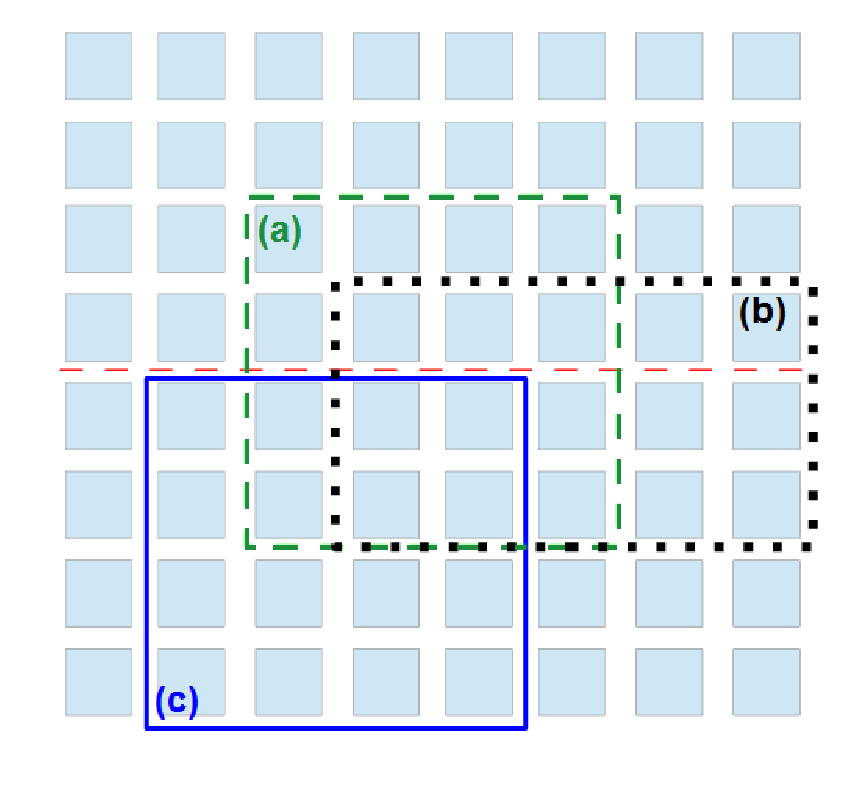
\includegraphics[width=0.75\linewidth]{bb_new.eps}
\caption{Illustration of three different scenarios for the wiring cost. The dashed green box shows a case where \textit{(a)} it crosses the interposer, the dotted black box shows a case where \textit{(b)} it barely crosses the cutline, and the solid blue one shows a case where \textit{(c)} the bounding box does not span the cutline.}
\label{fig:bb_illustration}
\end{figure}


\subsection{Router Optimization}
\label{sec:router_optimizations}
Once the Routing Resource Graph is modified as detailed in Section \ref{archSection}, the VPR router adapted automatically to the interposer architecture. The router starts at a net source node and expands by discovering adjacent routing nodes until it reaches the destination node. At any point, the router knows the cost of the path taken to the current point and it uses a \textit{lookahead cost function} to estimate the resource and delay cost from the current node to the destination. Using this lookahead cost, the router can properly sort routing alternatives. The lookahead cost function in VPR is not aware of the interposer, and therefore it takes a long time to converge to a routing decision. To make the lookahead aware of the interposer, we modify the lookahead cost function by adding terms that account for extra \textit{interposer delay} and extra \textit{interposer nodes} that may exist on the route from the current node to the destination node.

The VPR router uses the following to calculate a cost for a routing node \textit{r} on the route from \textit{i} to \textit{j}:
\setlength{\arraycolsep}{0.0em}
\begin{multline}
\label{eq:routing_cost}
Cost(r) = Criticality(i,j) \times Delay_{Elmore}(r, topology) \\ + [1-Criticality(i,j)] \times Congestion(r)
\end{multline}
\setlength{\arraycolsep}{5pt}

Given this cost function, the router's lookahead algorithm determines the total cost of the route from \textit{i} to \textit{j} when routing node \textit{r} is used:

\setlength{\arraycolsep}{0.0em}
\begin{multline}
\label{eq:lookahead_cost}
Cost_{Tot}(r) = \sum_{\forall l \in RT(i,r)} Cost(l) + \alpha \times ExpectCost(r,j)
\end{multline}
\setlength{\arraycolsep}{5pt}

where \textit{RT(i,r)} is the set of all routing nodes used so far from \textit{i} to \textit{r} and $\alpha$ is a constant number that determines the aggressiveness of the directed search. $\alpha$ is 1.2 by default in VPR. VPR's original $ExpectCost(n,j)$ function is~\cite{betz1999architecture}: 

\setlength{\arraycolsep}{0.0em}
\begin{multline}
\label{eq:expected_routing_cost}
ExpectCost(r,j) = Criticality_{fac} \times T_{del} + \\(1 - Criticality_{fac}) \times ExpectCongestionCost(r,j)
\end{multline}
\setlength{\arraycolsep}{5pt}

$T_{del}$ is an estimate of the delay that the router predicts it will see on the route from \textit{r} to \textit{j}. Since (\ref{eq:expected_routing_cost}) assumes a homogeneous FPGA, $T_{del}$ does not include the additional delay some routes experience by going through the interposer. Thus, for interposer-based architectures, we replace $T_{del}$ in (\ref{eq:expected_routing_cost}) with $T^\prime_{del}$ to include the delay of expected interposer hops from \textit{r} to \textit{j}.

\begin{multline}
\label{eq:tdelay}
T^\prime_{del} = T_{del} + T_{interposer} \times NumExpectedInterpHops
\end{multline}
\setlength{\arraycolsep}{5pt}

We modify $ExpectCongestionCost(r,j)$ in (\ref{eq:expected_routing_cost}) in a similar way to account for the new interposer routing nodes. 

The interposer-aware router lookahead makes routing decisions more quickly given the large delay difference of a path that crosses the interposer as opposed to a path that doesn't.

%   - Effectiveness / results
\subsection{Effectiveness of the Enhancements}
\label{sec:CADeffect}
For all experiments in this paper, the remaining architecture parameters of the FPGA are taken from the ``flagship" architecture of the VTR project (\textit{k6\_frac\_N10\_mem32K\_40nm.xml}) \cite{luu2014vtr}. The parameters of this architecture are in line with both current commercial FPGAs and academic research into best practices. It consists of logic clusters with 10 fracturable 6-LUTs per block (N=10, k=6), and also includes 32kb RAM blocks and DSP blocks configurable to perform 9x9, 18x18 or 36x36 multipliers. The delay values in the architecture are taken from 40 nm circuit simulations and 40 nm commercial FPGAs. It uses unidirectional routing, with all wire segments having length L = 4.

We used VPR 7.0, with the enhancements we detailed above, and the architecture file \textit{k6\_frac\_N10\_mem32K\_40nm} in the experiments below. All experiments targeted the smallest FPGA (with number of rows equal to number of columns) which could accommodate a benchmark circuit; this represents a very full FPGA with little white space left, and hence presents a difficult case to an interposer-based FPGA as no die can be left mostly empty. 

We have used the eight largest circuits from the VTR benchmark~\cite{vtr2012}, namely: \textit{bgm}, \textit{LU8PEEng}, \textit{LU32PEEng}, \textit{mcml}, \textit{mkDelayWorker32B}, \textit{stereovision0}, \textit{stereovision1} and \textit{stereovision2}. The size of these circuits ranges from $9,100$ to $153,000$ primitives (LUTs, FFs, etc.), with an average size of $52,600$ primitives. All results are the geometric mean over all circuits for a given interposer architecture.

To obtain the \textit{critical path delay} the circuits were run with a low stress routing with a channel width, $W = 1.3 \times minW$, where $minW$ is the minimum channel width for which the circuit is still routable. 

\subsubsection{Effectiveness of Placer Optimizations}
\label{sec:effectiveness_of_placer_enhancements}
Enabling the enhancements described in Section~\ref{cad_enh_placer_subsection} improves both the minimum routable channel width and circuit speed. As shown in Figure~\ref{fig:comparison_minW}, for architectures with low \textit{\% wires cut} (high interposer capacity), the placer optimizations have only a marginal benefit on routability compared to the original VPR placer since the interposer wires are not scarce, but as more wires are cut and we reach the realistic interposer capacity of commercial FPGAs, the placer optimizations provide higher and higher reductions in minimum channel width. When 80\% of wires are cut, the placer optimizations result in 11.3\% reduction in minimum channel width.

\begin{figure}[!htbp]
\centering
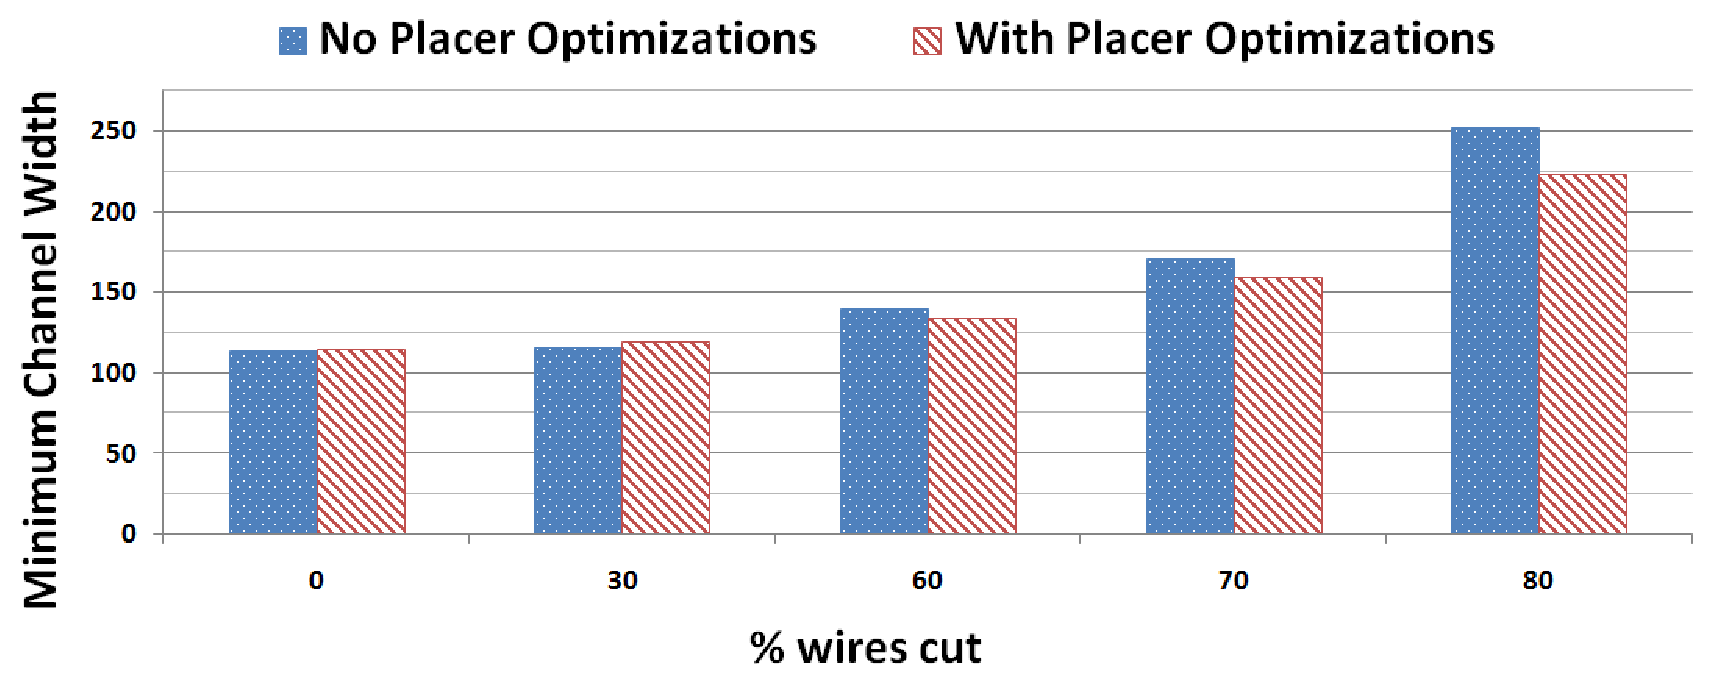
\includegraphics[width=\linewidth]{placer_opt_minChW_2.eps}
\caption{Impact of placer optimizations on minimum channel width.}
\label{fig:comparison_minW}
\end{figure}

The optimizations also guide the placer to keep related entities on the same die to reduce the number of inter-die signal crossings and hence increase circuit speed. This speed improvement is fairly consistent across a wide range of \%~wires~cut, averaging 12.5\% higher circuit speed.
\begin{figure}[!htbp]
\centering
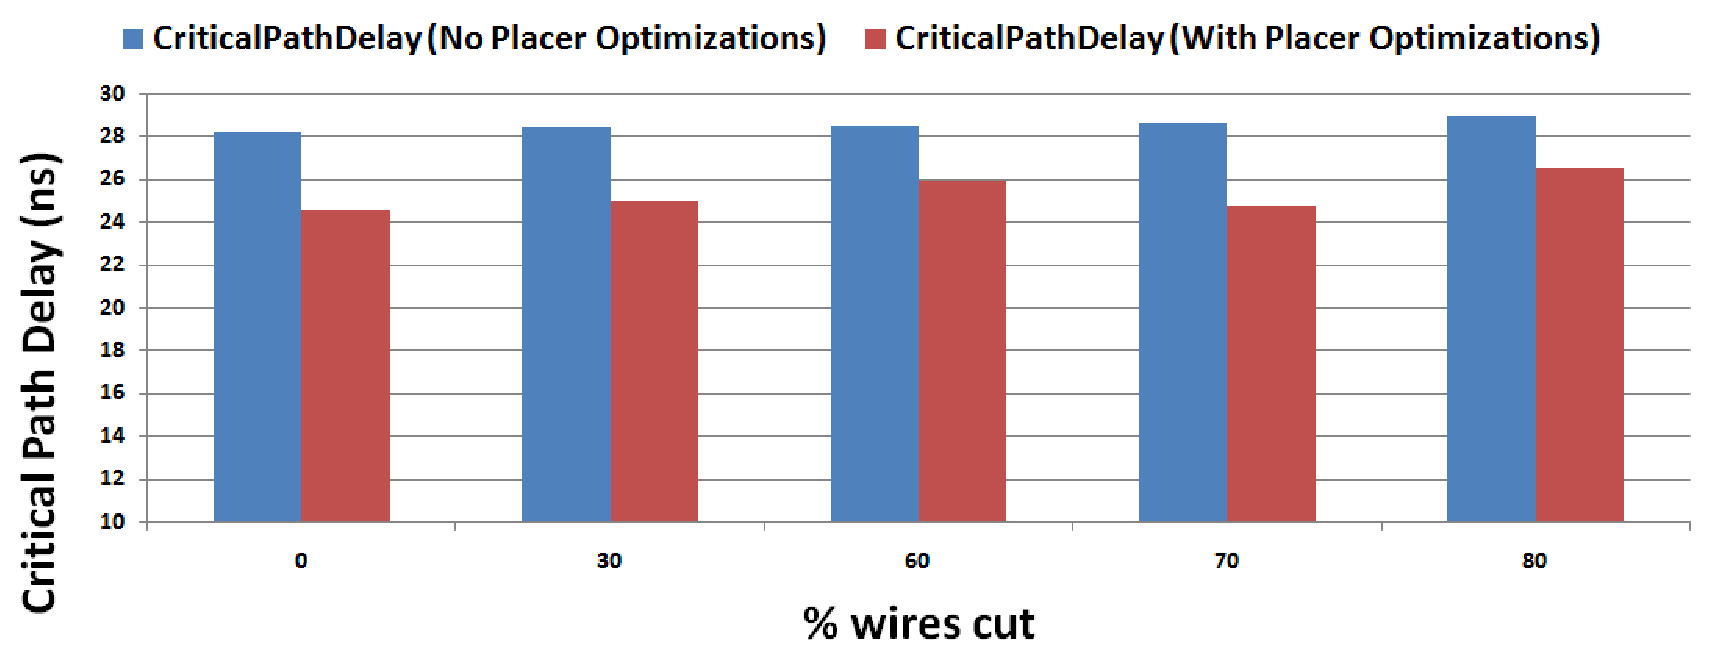
\includegraphics[width=\linewidth]{placer_opt_fmax.eps}
\caption{Impact of placer optimizations on circuit speed.}
\label{fig:comparison_fmax}
\end{figure}

\subsubsection{Effectiveness of Router Optimizations}
\label{sec:effectiveness_of_router_enhancements}
The router optimizations described in Section~\ref{sec:router_optimizations} greatly reduce the runtime of the router. Figure~\ref{fig:lookahead_runtime} shows the geomean of the router runtime for the 8 largest VTR circuits for different \textit{\% wires cut} values. On average, the router runs 31 times faster and finds identical minimum channel widths for all circuits.

\begin{figure}[!hb]
\centering
\includegraphics[width=\linewidth]{router_opt.eps}
\caption{Router runtime with original and updated lookahead function.}
\label{fig:lookahead_runtime}
\end{figure}

The new router lookahead changes the priority of the routes discovered by the router. Using the new router lookahead function increases the critical path delay by 1.3\% on average. We consider this small quality loss acceptable and use the enhanced router lookahead in all our experiments due to its greatly reduced runtime.

%---------------------------------------------------------------
%---------------------------------------------------------------
%---------------------------------------------------------------
\section{Adding Partitioning to the CAD Flow}
\label{sec:CADflow}
Given that the number of signals that can cross the interposer between FPGA dice is considerably more limited than within an FPGA, using a partitioner to divide the circuit into one partition per die is a promising CAD flow.

\subsection{CAD Flow Variations}
The overall CAD flow, including the partitioning steps, is shown in Figure \ref{fig:partitioning_cad_flow}.
\begin{figure}[!htbp]
\centering
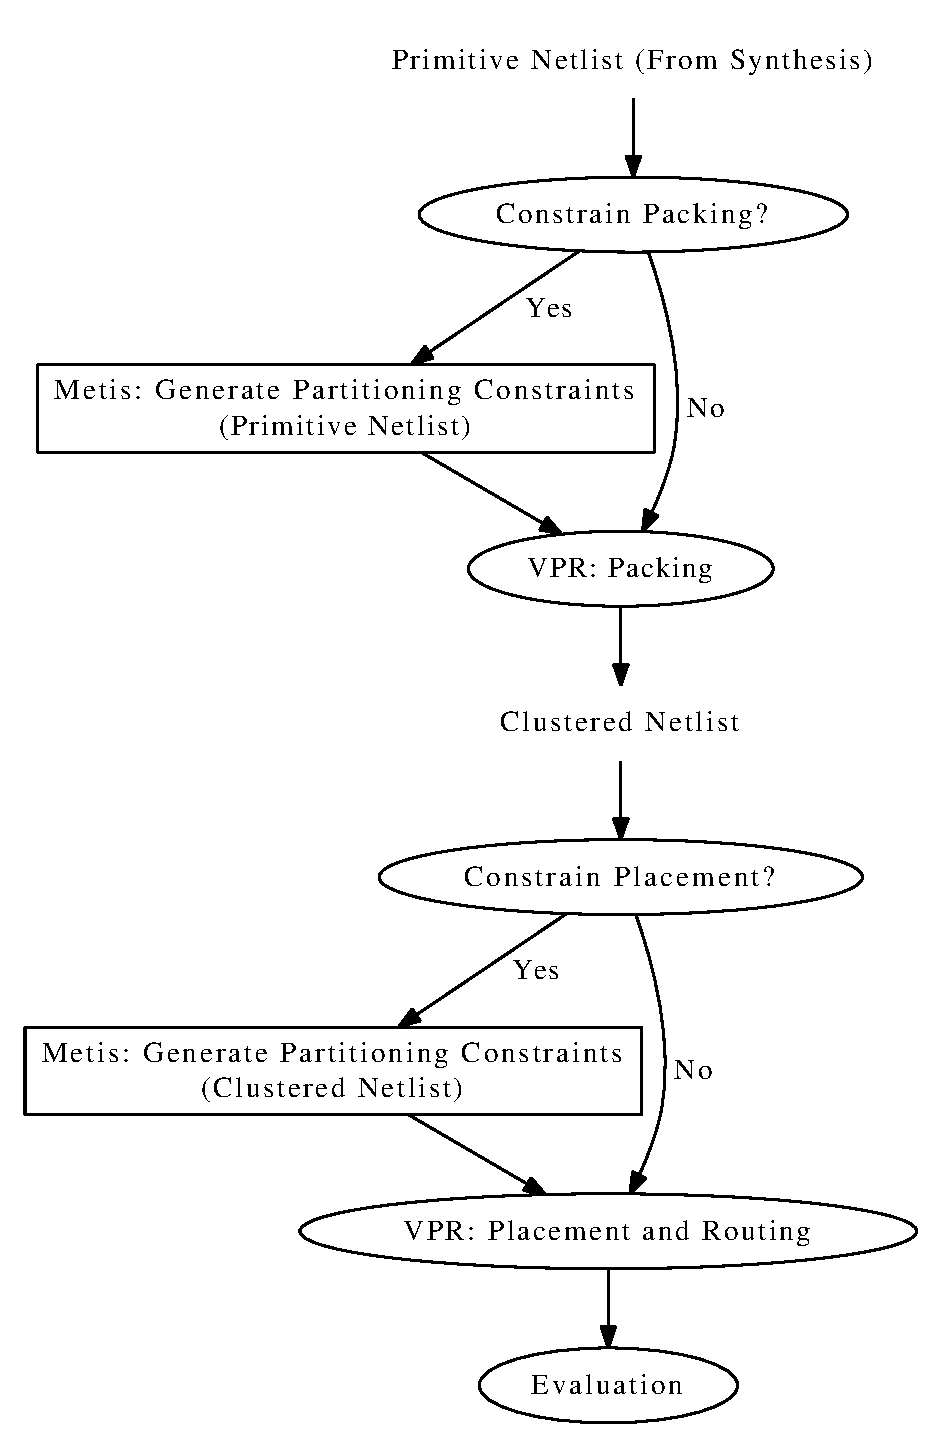
\includegraphics[height=3.5in]{partitioning_cad_flow.eps}
\caption{Possible ways to add partitioning to the VPR CAD flow.}
\label{fig:partitioning_cad_flow}
\end{figure}

\subsubsection{Partitioner Stage}\label{sec:partitioner_stage}
As shown in Figure \ref{fig:partitioning_cad_flow}, we explore the effect of circuit partitioning at two different stages of the CAD flow. The first possibility is to partition the netlist of primitive elements (LUTs, FFs, RAM slices, etc.) before packing into the larger function blocks such as logic blocks and (32 kb) RAM blocks. The partitioning constraints must be respected by the packer; it must not pack two primitives assigned to different partitions (dice) into the same function block. We updated the VPR clustering algorithm to respect this new constraint. The second possible way to incorporate partitioning is after packing, where partitioning is applied to the function block (cluster-level) netlist. Each partition is then assigned (randomly) to a separate FPGA die. The partitioning constraints must then be respected by the placer; it is free to move function blocks around within a die, but not across interposer cutlines. These two partitioning flow options can be combined -- if partitioning is applied before packing, one can also pass the partition information to the placement stage. The post-packing placement constraints can be derived from the primitive block partitioning constraints, with the valid placement region for a given function block being equal to the intersection of the valid placement regions of the primitives packed into that function (clustered) block. There are, therefore, four possible partitioning flows:

\begin{enumerate}
  \item Leaving both the packer and the placer unconstrained. This is the base flow that does not use partitioning, as described in Section \ref{cadSection}.
  \item Partitioning the primitive netlist to guide the packer, leaving the placer unconstrained.
  \item Leaving the packer unconstrained, and partitioning the function block (clustered) netlist to guide the placer.
  \item Partitioning the primitive netlist to guide the packer, and constraining the placer based on constraints derived from partitioning, as described above.
\end{enumerate}

\subsubsection{Partitioning Tool}
Two well-known freely available graph partitioning tools are Metis~\cite{karypis1998multilevelmetis} and hMetis~\cite{karypis1999multilevelhmetis}. Metis operates on graphs, while hMetis operates on hypergraphs -- a hypergraph is a generalization of a graph, where each edge can connect any number of vertices. It is most natural to represent a circuit netlist as a hypergraph, where the vertices are netlist pins (or blocks) and the hyperedges are the nets joining the pins. Based on that criterion alone, hMetis would be the most appropriate choice of partitioner. However, there are other important criteria to consider for our use case.

Graph partitioning algorithms generate partitions of a circuit while satisfying ``balance constraints''. The balance constraints exist to drive the algorithm away from the trivial partitioning solution where all vertices are in the same partition, leaving all other partitions empty. An example of a basic balance constraint is one which requires an equal number of vertices in each partition. Generally such a perfect balance overly restricts the solution, so some fractional ``unbalance'' is allowed; in this work we use $0.05$ ($5\%$). For two partitions, $P1$ and $P2$, this translates to~\cite{karypismanual}

\begin{equation}\label{eq:balance_constraint}
\frac{|P1|}{|P1 \cup P2|} \in [0.5 - unbalance, 0.5 + unbalance]
\end{equation}

To derive an appropriate balance constraint for our use case, consider that FPGA circuit netlists may contain different block types such as LUTs, registers, RAM slices, and multipliers, among others. The basic balance constraint of (\ref{eq:balance_constraint}), applied to the two partition case with only LUTs and multipliers would ensure that the total block count (sum of the LUT count + multiplier count) in each partition is roughly balanced.

The problem with (\ref{eq:balance_constraint}) in the case of multiple block types is that the capacity of each partition is not taken into account on a per-block-type basis. It is therefore possible to generate partitions that cannot be realized because the number of resources of each type is not balanced across partitions, even though the total number of resources is balanced. For example, there is nothing preventing the partitioner from moving all LUTs to partition 1 and all multipliers to partition 2, which would not be physically realizable because partition 1 may not have enough LUTs to implement the desired partitioning (and no LUTs in partition 2 would be used.) One solution is to enforce a balance constraint on each block type, $i$:

\begin{equation}
\forall i, \abs*{ \frac{| P1_i |}{|P1_i \cup P2_i |} - 0.5} < unbalance
\end{equation}
where $P1_i$ is the set of all blocks of type $i$ in partition 1.

We refer to this type of per-block set of constraints as heterogeneous balance constraints. Note that there are complex legality constraints governing which LUTs and FFs can be packed into legal logic blocks, as well as which multipliers can be packed into legal DSP blocks~\cite{luu2014vtr}. As the partitioner is not aware of these constraints, flow 3 above (which runs the partitioner after function block packing) will be able to more precisely balance resource use across partitions.

The latest public version of hMetis does not support heterogeneous balance constraints, though Metis does. Metis was used in our CAD flow. However, as discussed earlier, the circuit netlist is most naturally represented as a hypergraph, and so it needs to be transformed to a graph before Metis can process it.

\subsubsection{Hypergraph to Graph Transformation}\label{sec:hypergraph_to_graph}
We transformed the circuit netlist hypergraph to a graph in the following way:
\begin{enumerate}
\item For each hyperedge of the circuit netlist hypergraph, we generated a graph (the \emph{per-net subgraph}).
\item We combined all of the per-net subgraphs, summing the edge weights for edges appearing in more than one per-net subgraph, to generate the total netlist graph.
\end{enumerate}

We explored several ways to generate the per-net subgraphs. The two parameters in this operation are the graph topology and the edge weight scheme. We considered two subgraph topologies, clique and star, as illustrated in Figure \ref{fig:star_clique}. We assigned the same edge weight to every edge of the generated subgraph. Edge weights were computed based on the number of vertices in the hyperedge, $n$, and we considered edge weights equal to $1$, $1/n$, and $1/n^2$.

\begin{figure}[!htbp]
\centering
\subfigure[]{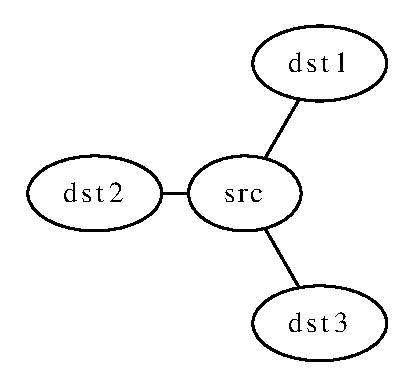
\includegraphics[width=0.45\linewidth]{star.eps}}
\subfigure[]{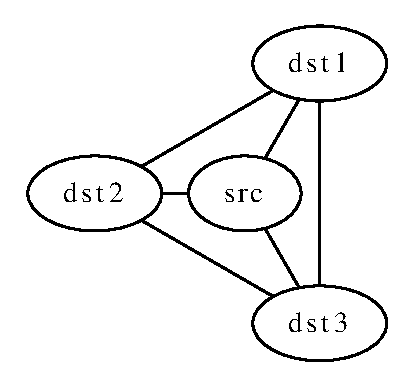
\includegraphics[width=0.45\linewidth]{clique.eps}}
\caption{(a) Star and (b) clique graph topologies.}
\label{fig:star_clique}
\end{figure}



Figure \ref{fig:hyperedge_to_graph} shows how a netlist of three blocks and two nets is transformed into its component subgraphs. TODO JAVEED: Maybe just show star 1/n from start to finish.

\begin{figure}[!htbp]
\centering
\subfigure[]{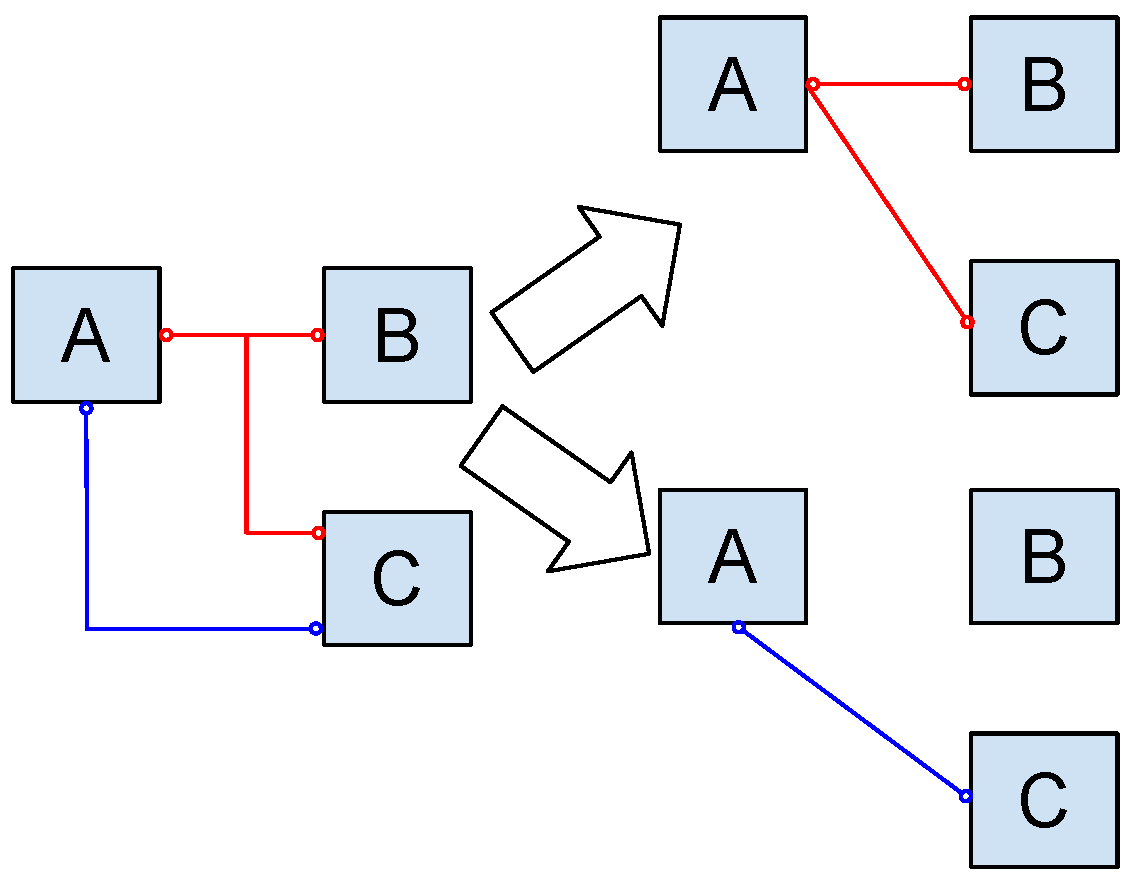
\includegraphics[width=0.45\linewidth]{hg2g_star.pdf}}
\subfigure[]{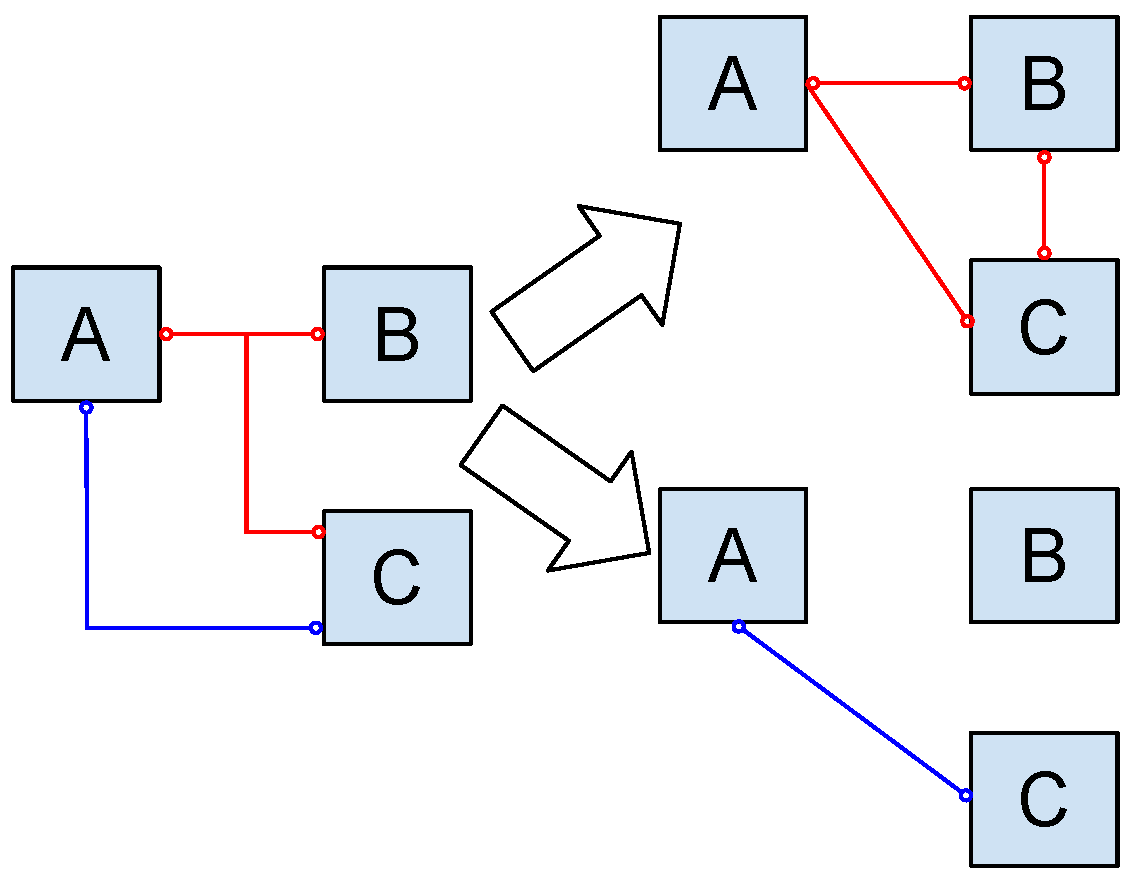
\includegraphics[width=0.45\linewidth]{hg2g_clique.pdf}}
\caption{The hypergraph to graph transformation with (a) the star topology, and (b) the clique topology.}
\label{fig:hyperedge_to_graph}
\end{figure}

The parameters of graph topology and edge weight were evaluated by generating the total primitive netlist graph and running it through the Metis partitioner to generate two partitions. The results of the different schemes were ranked based on the hyperedge cutsize, which is the number of hyperedges crossing the cutline, as illustrated in Figure \ref{fig:hyperedge_cutline}. The hyperedge cutsize is a proxy for the routability of the circuit, as the cutsize is the number of nets that cross the interposer boundary. To compute the hyperedge cutsize, we applied the partitioning result (which assigns each vertex to a partition number) to the original untransformed hypergraph, and counted the number of hyperedges whose vertices were spread across different partitions. We computed the hyperedge cutsize for every combination of graph topology and graph edge weight scheme, across several circuits. The results are shown in Figure \ref{fig:graph_topology_cutsize}.

\begin{figure}[!htbp]
\centering
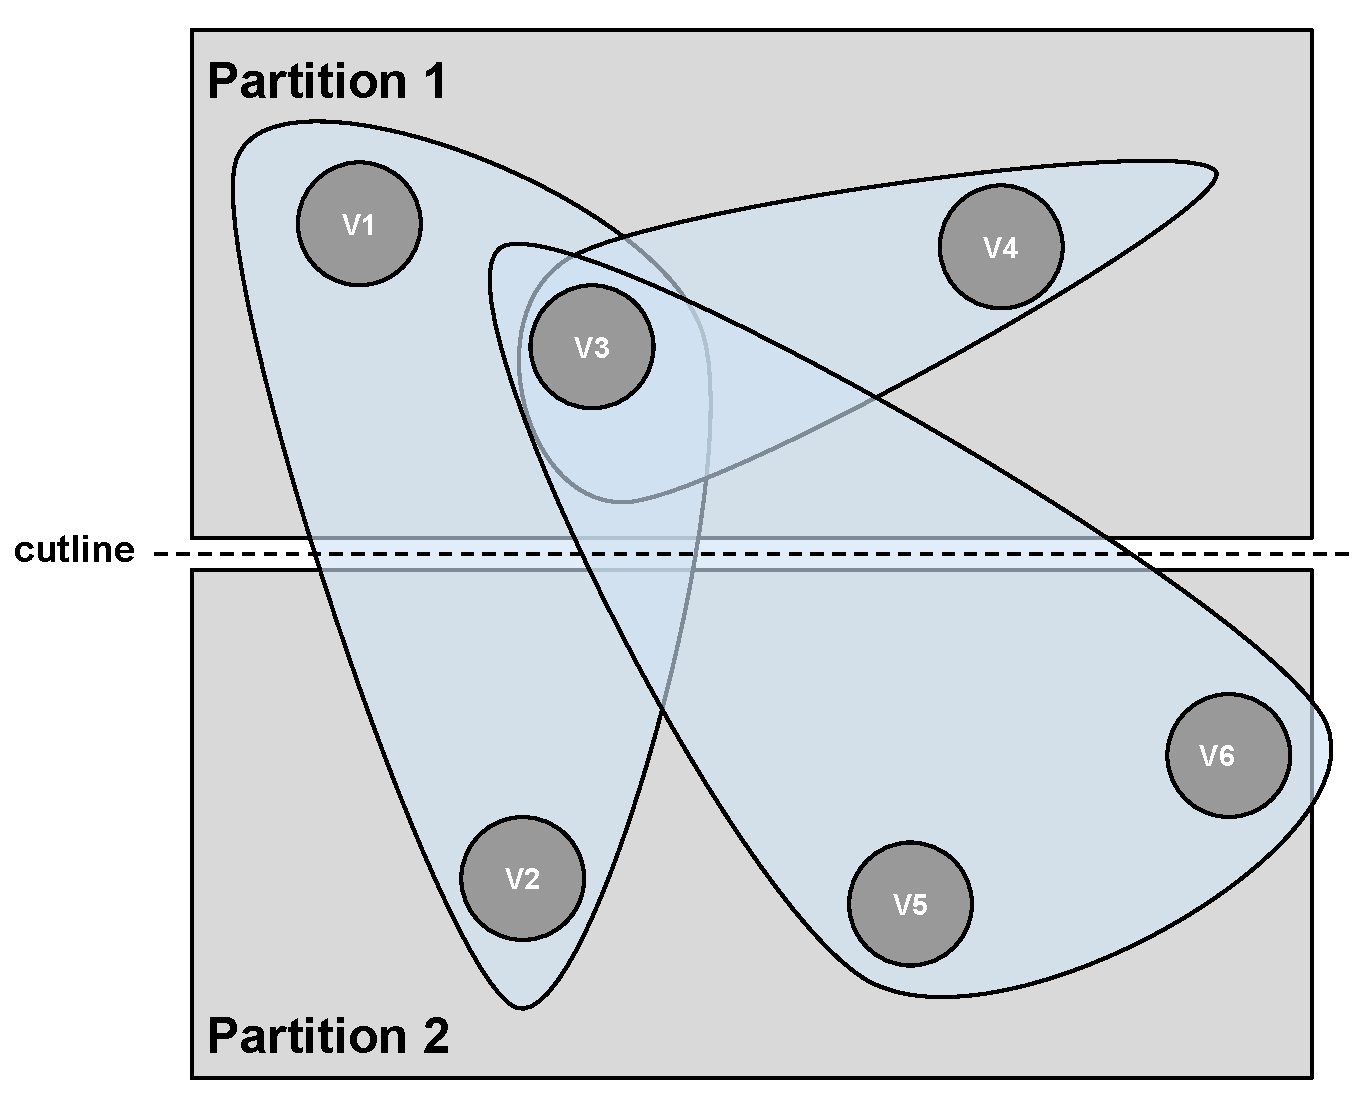
\includegraphics[width=\linewidth]{hyperedge_cutline.pdf}
\caption{A graph with six vertices and three hyperedges partitioned into two halves. As there are two hyperedges crossing the cutline, the hyperedge cutsize is 2.}
\label{fig:hyperedge_cutline}
\end{figure}

\begin{figure}[!htbp]
\centering
%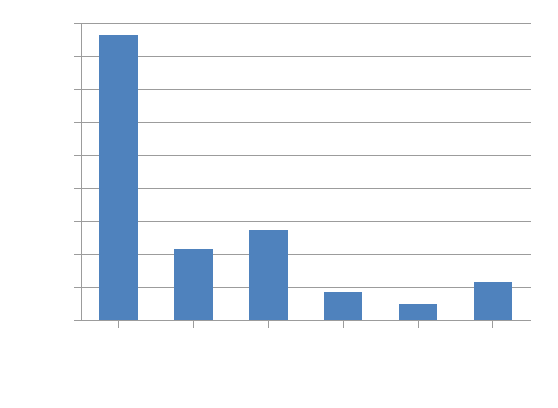
\includegraphics[width=\linewidth]{graph_topology_cutsize.eps}
%% GNUPLOT: LaTeX picture with Postscript
\begingroup
  \makeatletter
  \providecommand\color[2][]{%
    \GenericError{(gnuplot) \space\space\space\@spaces}{%
      Package color not loaded in conjunction with
      terminal option `colourtext'%
    }{See the gnuplot documentation for explanation.%
    }{Either use 'blacktext' in gnuplot or load the package
      color.sty in LaTeX.}%
    \renewcommand\color[2][]{}%
  }%
  \providecommand\includegraphics[2][]{%
    \GenericError{(gnuplot) \space\space\space\@spaces}{%
      Package graphicx or graphics not loaded%
    }{See the gnuplot documentation for explanation.%
    }{The gnuplot epslatex terminal needs graphicx.sty or graphics.sty.}%
    \renewcommand\includegraphics[2][]{}%
  }%
  \providecommand\rotatebox[2]{#2}%
  \@ifundefined{ifGPcolor}{%
    \newif\ifGPcolor
    \GPcolortrue
  }{}%
  \@ifundefined{ifGPblacktext}{%
    \newif\ifGPblacktext
    \GPblacktexttrue
  }{}%
  % define a \g@addto@macro without @ in the name:
  \let\gplgaddtomacro\g@addto@macro
  % define empty templates for all commands taking text:
  \gdef\gplbacktext{}%
  \gdef\gplfronttext{}%
  \makeatother
  \ifGPblacktext
    % no textcolor at all
    \def\colorrgb#1{}%
    \def\colorgray#1{}%
  \else
    % gray or color?
    \ifGPcolor
      \def\colorrgb#1{\color[rgb]{#1}}%
      \def\colorgray#1{\color[gray]{#1}}%
      \expandafter\def\csname LTw\endcsname{\color{white}}%
      \expandafter\def\csname LTb\endcsname{\color{black}}%
      \expandafter\def\csname LTa\endcsname{\color{black}}%
      \expandafter\def\csname LT0\endcsname{\color[rgb]{1,0,0}}%
      \expandafter\def\csname LT1\endcsname{\color[rgb]{0,1,0}}%
      \expandafter\def\csname LT2\endcsname{\color[rgb]{0,0,1}}%
      \expandafter\def\csname LT3\endcsname{\color[rgb]{1,0,1}}%
      \expandafter\def\csname LT4\endcsname{\color[rgb]{0,1,1}}%
      \expandafter\def\csname LT5\endcsname{\color[rgb]{1,1,0}}%
      \expandafter\def\csname LT6\endcsname{\color[rgb]{0,0,0}}%
      \expandafter\def\csname LT7\endcsname{\color[rgb]{1,0.3,0}}%
      \expandafter\def\csname LT8\endcsname{\color[rgb]{0.5,0.5,0.5}}%
    \else
      % gray
      \def\colorrgb#1{\color{black}}%
      \def\colorgray#1{\color[gray]{#1}}%
      \expandafter\def\csname LTw\endcsname{\color{white}}%
      \expandafter\def\csname LTb\endcsname{\color{black}}%
      \expandafter\def\csname LTa\endcsname{\color{black}}%
      \expandafter\def\csname LT0\endcsname{\color{black}}%
      \expandafter\def\csname LT1\endcsname{\color{black}}%
      \expandafter\def\csname LT2\endcsname{\color{black}}%
      \expandafter\def\csname LT3\endcsname{\color{black}}%
      \expandafter\def\csname LT4\endcsname{\color{black}}%
      \expandafter\def\csname LT5\endcsname{\color{black}}%
      \expandafter\def\csname LT6\endcsname{\color{black}}%
      \expandafter\def\csname LT7\endcsname{\color{black}}%
      \expandafter\def\csname LT8\endcsname{\color{black}}%
    \fi
  \fi
  \setlength{\unitlength}{0.0500bp}%
  \begin{picture}(5040.00,3600.00)%
    \gplgaddtomacro\gplbacktext{%
      \colorrgb{0.61,0.61,0.61}%
      \put(510,680){\makebox(0,0)[r]{\strut{}\footnotesize{0}}}%
      \colorrgb{0.61,0.61,0.61}%
      \put(510,996){\makebox(0,0)[r]{\strut{}\footnotesize{500}}}%
      \colorrgb{0.61,0.61,0.61}%
      \put(510,1313){\makebox(0,0)[r]{\strut{}\footnotesize{1000}}}%
      \colorrgb{0.61,0.61,0.61}%
      \put(510,1629){\makebox(0,0)[r]{\strut{}\footnotesize{1500}}}%
      \colorrgb{0.61,0.61,0.61}%
      \put(510,1945){\makebox(0,0)[r]{\strut{}\footnotesize{2000}}}%
      \colorrgb{0.61,0.61,0.61}%
      \put(510,2262){\makebox(0,0)[r]{\strut{}\footnotesize{2500}}}%
      \colorrgb{0.61,0.61,0.61}%
      \put(510,2578){\makebox(0,0)[r]{\strut{}\footnotesize{3000}}}%
      \colorrgb{0.61,0.61,0.61}%
      \put(510,2894){\makebox(0,0)[r]{\strut{}\footnotesize{3500}}}%
      \colorrgb{0.61,0.61,0.61}%
      \put(510,3211){\makebox(0,0)[r]{\strut{}\footnotesize{4000}}}%
      \colorrgb{0.61,0.61,0.61}%
      \put(510,3527){\makebox(0,0)[r]{\strut{}\footnotesize{4500}}}%
      \colorrgb{0.61,0.61,0.61}%
      \put(977,521){\rotatebox{45}{\makebox(0,0)[r]{\strut{}\footnotesize{clique $1$}}}}%
      \colorrgb{0.61,0.61,0.61}%
      \put(1696,521){\rotatebox{45}{\makebox(0,0)[r]{\strut{}\footnotesize{clique $1/n$}}}}%
      \colorrgb{0.61,0.61,0.61}%
      \put(2415,521){\rotatebox{45}{\makebox(0,0)[r]{\strut{}\footnotesize{clique $1/n^2$}}}}%
      \colorrgb{0.61,0.61,0.61}%
      \put(3134,521){\rotatebox{45}{\makebox(0,0)[r]{\strut{}\footnotesize{star $1$}}}}%
      \colorrgb{0.61,0.61,0.61}%
      \put(3853,521){\rotatebox{45}{\makebox(0,0)[r]{\strut{}\footnotesize{star $1/n$}}}}%
      \colorrgb{0.61,0.61,0.61}%
      \put(4572,521){\rotatebox{45}{\makebox(0,0)[r]{\strut{}\footnotesize{star $1/n^2$}}}}%
      \csname LTb\endcsname%
      \put(48,2103){\rotatebox{-270}{\makebox(0,0){\strut{}\footnotesize{\textbf{Hyperedge Cut Size}}}}}%
      \put(2774,42){\makebox(0,0){\strut{}\footnotesize{\textbf{Graph Topology}}}}%
    }%
    \gplgaddtomacro\gplfronttext{%
    }%
    \gplbacktext
    \put(0,0){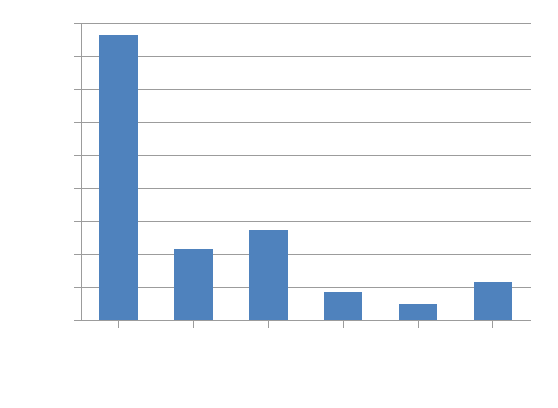
\includegraphics{graph_topology_cutsize}}%
    \gplfronttext
  \end{picture}%
\endgroup

% GNUPLOT: LaTeX picture with Postscript
\begingroup
  \makeatletter
  \providecommand\color[2][]{%
    \GenericError{(gnuplot) \space\space\space\@spaces}{%
      Package color not loaded in conjunction with
      terminal option `colourtext'%
    }{See the gnuplot documentation for explanation.%
    }{Either use 'blacktext' in gnuplot or load the package
      color.sty in LaTeX.}%
    \renewcommand\color[2][]{}%
  }%
  \providecommand\includegraphics[2][]{%
    \GenericError{(gnuplot) \space\space\space\@spaces}{%
      Package graphicx or graphics not loaded%
    }{See the gnuplot documentation for explanation.%
    }{The gnuplot epslatex terminal needs graphicx.sty or graphics.sty.}%
    \renewcommand\includegraphics[2][]{}%
  }%
  \providecommand\rotatebox[2]{#2}%
  \@ifundefined{ifGPcolor}{%
    \newif\ifGPcolor
    \GPcolortrue
  }{}%
  \@ifundefined{ifGPblacktext}{%
    \newif\ifGPblacktext
    \GPblacktexttrue
  }{}%
  % define a \g@addto@macro without @ in the name:
  \let\gplgaddtomacro\g@addto@macro
  % define empty templates for all commands taking text:
  \gdef\gplbacktext{}%
  \gdef\gplfronttext{}%
  \makeatother
  \ifGPblacktext
    % no textcolor at all
    \def\colorrgb#1{}%
    \def\colorgray#1{}%
  \else
    % gray or color?
    \ifGPcolor
      \def\colorrgb#1{\color[rgb]{#1}}%
      \def\colorgray#1{\color[gray]{#1}}%
      \expandafter\def\csname LTw\endcsname{\color{white}}%
      \expandafter\def\csname LTb\endcsname{\color{black}}%
      \expandafter\def\csname LTa\endcsname{\color{black}}%
      \expandafter\def\csname LT0\endcsname{\color[rgb]{1,0,0}}%
      \expandafter\def\csname LT1\endcsname{\color[rgb]{0,1,0}}%
      \expandafter\def\csname LT2\endcsname{\color[rgb]{0,0,1}}%
      \expandafter\def\csname LT3\endcsname{\color[rgb]{1,0,1}}%
      \expandafter\def\csname LT4\endcsname{\color[rgb]{0,1,1}}%
      \expandafter\def\csname LT5\endcsname{\color[rgb]{1,1,0}}%
      \expandafter\def\csname LT6\endcsname{\color[rgb]{0,0,0}}%
      \expandafter\def\csname LT7\endcsname{\color[rgb]{1,0.3,0}}%
      \expandafter\def\csname LT8\endcsname{\color[rgb]{0.5,0.5,0.5}}%
    \else
      % gray
      \def\colorrgb#1{\color{black}}%
      \def\colorgray#1{\color[gray]{#1}}%
      \expandafter\def\csname LTw\endcsname{\color{white}}%
      \expandafter\def\csname LTb\endcsname{\color{black}}%
      \expandafter\def\csname LTa\endcsname{\color{black}}%
      \expandafter\def\csname LT0\endcsname{\color{black}}%
      \expandafter\def\csname LT1\endcsname{\color{black}}%
      \expandafter\def\csname LT2\endcsname{\color{black}}%
      \expandafter\def\csname LT3\endcsname{\color{black}}%
      \expandafter\def\csname LT4\endcsname{\color{black}}%
      \expandafter\def\csname LT5\endcsname{\color{black}}%
      \expandafter\def\csname LT6\endcsname{\color{black}}%
      \expandafter\def\csname LT7\endcsname{\color{black}}%
      \expandafter\def\csname LT8\endcsname{\color{black}}%
    \fi
  \fi
  \setlength{\unitlength}{0.0500bp}%
  \begin{picture}(5040.00,3600.00)%
    \gplgaddtomacro\gplbacktext{%
      \colorrgb{0.61,0.61,0.61}%
      \put(510,680){\makebox(0,0)[r]{\strut{}\footnotesize{0}}}%
      \colorrgb{0.61,0.61,0.61}%
      \put(510,996){\makebox(0,0)[r]{\strut{}\footnotesize{500}}}%
      \colorrgb{0.61,0.61,0.61}%
      \put(510,1313){\makebox(0,0)[r]{\strut{}\footnotesize{1000}}}%
      \colorrgb{0.61,0.61,0.61}%
      \put(510,1629){\makebox(0,0)[r]{\strut{}\footnotesize{1500}}}%
      \colorrgb{0.61,0.61,0.61}%
      \put(510,1945){\makebox(0,0)[r]{\strut{}\footnotesize{2000}}}%
      \colorrgb{0.61,0.61,0.61}%
      \put(510,2262){\makebox(0,0)[r]{\strut{}\footnotesize{2500}}}%
      \colorrgb{0.61,0.61,0.61}%
      \put(510,2578){\makebox(0,0)[r]{\strut{}\footnotesize{3000}}}%
      \colorrgb{0.61,0.61,0.61}%
      \put(510,2894){\makebox(0,0)[r]{\strut{}\footnotesize{3500}}}%
      \colorrgb{0.61,0.61,0.61}%
      \put(510,3211){\makebox(0,0)[r]{\strut{}\footnotesize{4000}}}%
      \colorrgb{0.61,0.61,0.61}%
      \put(510,3527){\makebox(0,0)[r]{\strut{}\footnotesize{4500}}}%
      \colorrgb{0.61,0.61,0.61}%
      \put(977,521){\rotatebox{45}{\makebox(0,0)[r]{\strut{}\footnotesize{clique $1$}}}}%
      \colorrgb{0.61,0.61,0.61}%
      \put(1696,521){\rotatebox{45}{\makebox(0,0)[r]{\strut{}\footnotesize{clique $1/n$}}}}%
      \colorrgb{0.61,0.61,0.61}%
      \put(2415,521){\rotatebox{45}{\makebox(0,0)[r]{\strut{}\footnotesize{clique $1/n^2$}}}}%
      \colorrgb{0.61,0.61,0.61}%
      \put(3134,521){\rotatebox{45}{\makebox(0,0)[r]{\strut{}\footnotesize{star $1$}}}}%
      \colorrgb{0.61,0.61,0.61}%
      \put(3853,521){\rotatebox{45}{\makebox(0,0)[r]{\strut{}\footnotesize{star $1/n$}}}}%
      \colorrgb{0.61,0.61,0.61}%
      \put(4572,521){\rotatebox{45}{\makebox(0,0)[r]{\strut{}\footnotesize{star $1/n^2$}}}}%
      \csname LTb\endcsname%
      \put(48,2103){\rotatebox{-270}{\makebox(0,0){\strut{}\footnotesize{\textbf{Hyperedge Cut Size}}}}}%
      \put(2774,42){\makebox(0,0){\strut{}\footnotesize{\textbf{Graph Topology}}}}%
    }%
    \gplgaddtomacro\gplfronttext{%
    }%
    \gplbacktext
    \put(0,0){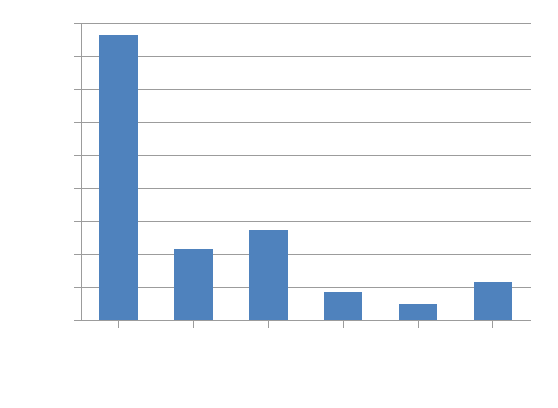
\includegraphics{graph_topology_cutsize}}%
    \gplfronttext
  \end{picture}%
\endgroup

\caption{Hypergraph cut size achieved by Metis with different hyperedge models and weightings. n is the number of vertices on a hyperedge.}
\label{fig:graph_topology_cutsize}
\end{figure}

The performance of the clique topology is significantly worse than that of the star topology, regardless of edge weight scheme. An intuitive explanation for this result is that with the clique topology, the partitioner does not have knowledge of which vertex is the source of a net and which vertices are sinks. In contrast, the star topology clearly differentiates sources from sinks and this appears to give the partitioner an “anchor point” that pulls all hyperedge fanouts toward the source. Additionally, if $n$ is the average number of vertices in a hyperedge, the clique topology generates $O(n^2)$ edges while the star topology generates only $O(n)$ edges, so the star topology saves both memory and runtime.

For both topologies, the $1/n$ edge weight scheme gives the smallest cut size on average. This can be explained intuitively in terms of the total edge weight over all edges of the graph. The star $1$ (constant) edge weight scheme assigns a total weight of $n$ to each net, which heavily weights high-fanout nets. In contrast, the star $1/n$ scheme assigns the same total weight of $1$ to each net. The star $1/n^2$ scheme penalizes high-fanout nets relative to lower-fanout nets. Since we seek to minimize the hyperedge cut, it makes intuitive sense to weight all hyperedges equally, and the star $1/n$ scheme achieves this.

To validate the choice of hyperedge cutsize as a proxy for circuit routability, we ran the partitioning CAD flow for each graph topology and edge weight scheme, across several circuits. We use an unbalance of $5\%$, split the clustered netlist into two partitions (constraining only the placer), cut $80\%$ of the wires crossing the interposer, and impose a $1ns$ delay penalty for wires crossing the interposer. To accommodate unbalance in the placement engine, we increase the size of the grid of complex blocks that make up the FPGA device. Relative to the minimum device size required for placement (without partitioning constraints), we add $10\%$ to the complex block grid width and $10\%$ to the grid height. Figure \ref{fig:graph_topology_mcw} shows the geometric mean of the minimum channel width required for a successful route, for each of the graph topology and edge weight combinations.

\begin{figure}[!htbp]
\centering
% GNUPLOT: LaTeX picture with Postscript
\begingroup
  \makeatletter
  \providecommand\color[2][]{%
    \GenericError{(gnuplot) \space\space\space\@spaces}{%
      Package color not loaded in conjunction with
      terminal option `colourtext'%
    }{See the gnuplot documentation for explanation.%
    }{Either use 'blacktext' in gnuplot or load the package
      color.sty in LaTeX.}%
    \renewcommand\color[2][]{}%
  }%
  \providecommand\includegraphics[2][]{%
    \GenericError{(gnuplot) \space\space\space\@spaces}{%
      Package graphicx or graphics not loaded%
    }{See the gnuplot documentation for explanation.%
    }{The gnuplot epslatex terminal needs graphicx.sty or graphics.sty.}%
    \renewcommand\includegraphics[2][]{}%
  }%
  \providecommand\rotatebox[2]{#2}%
  \@ifundefined{ifGPcolor}{%
    \newif\ifGPcolor
    \GPcolortrue
  }{}%
  \@ifundefined{ifGPblacktext}{%
    \newif\ifGPblacktext
    \GPblacktexttrue
  }{}%
  % define a \g@addto@macro without @ in the name:
  \let\gplgaddtomacro\g@addto@macro
  % define empty templates for all commands taking text:
  \gdef\gplbacktext{}%
  \gdef\gplfronttext{}%
  \makeatother
  \ifGPblacktext
    % no textcolor at all
    \def\colorrgb#1{}%
    \def\colorgray#1{}%
  \else
    % gray or color?
    \ifGPcolor
      \def\colorrgb#1{\color[rgb]{#1}}%
      \def\colorgray#1{\color[gray]{#1}}%
      \expandafter\def\csname LTw\endcsname{\color{white}}%
      \expandafter\def\csname LTb\endcsname{\color{black}}%
      \expandafter\def\csname LTa\endcsname{\color{black}}%
      \expandafter\def\csname LT0\endcsname{\color[rgb]{1,0,0}}%
      \expandafter\def\csname LT1\endcsname{\color[rgb]{0,1,0}}%
      \expandafter\def\csname LT2\endcsname{\color[rgb]{0,0,1}}%
      \expandafter\def\csname LT3\endcsname{\color[rgb]{1,0,1}}%
      \expandafter\def\csname LT4\endcsname{\color[rgb]{0,1,1}}%
      \expandafter\def\csname LT5\endcsname{\color[rgb]{1,1,0}}%
      \expandafter\def\csname LT6\endcsname{\color[rgb]{0,0,0}}%
      \expandafter\def\csname LT7\endcsname{\color[rgb]{1,0.3,0}}%
      \expandafter\def\csname LT8\endcsname{\color[rgb]{0.5,0.5,0.5}}%
    \else
      % gray
      \def\colorrgb#1{\color{black}}%
      \def\colorgray#1{\color[gray]{#1}}%
      \expandafter\def\csname LTw\endcsname{\color{white}}%
      \expandafter\def\csname LTb\endcsname{\color{black}}%
      \expandafter\def\csname LTa\endcsname{\color{black}}%
      \expandafter\def\csname LT0\endcsname{\color{black}}%
      \expandafter\def\csname LT1\endcsname{\color{black}}%
      \expandafter\def\csname LT2\endcsname{\color{black}}%
      \expandafter\def\csname LT3\endcsname{\color{black}}%
      \expandafter\def\csname LT4\endcsname{\color{black}}%
      \expandafter\def\csname LT5\endcsname{\color{black}}%
      \expandafter\def\csname LT6\endcsname{\color{black}}%
      \expandafter\def\csname LT7\endcsname{\color{black}}%
      \expandafter\def\csname LT8\endcsname{\color{black}}%
    \fi
  \fi
  \setlength{\unitlength}{0.0500bp}%
  \begin{picture}(5040.00,2160.00)%
    \gplgaddtomacro\gplbacktext{%
      \colorrgb{0.61,0.61,0.61}%
      \put(474,680){\makebox(0,0)[r]{\strut{}\footnotesize{160}}}%
      \colorrgb{0.61,0.61,0.61}%
      \put(474,915){\makebox(0,0)[r]{\strut{}\footnotesize{180}}}%
      \colorrgb{0.61,0.61,0.61}%
      \put(474,1149){\makebox(0,0)[r]{\strut{}\footnotesize{200}}}%
      \colorrgb{0.61,0.61,0.61}%
      \put(474,1384){\makebox(0,0)[r]{\strut{}\footnotesize{220}}}%
      \colorrgb{0.61,0.61,0.61}%
      \put(474,1618){\makebox(0,0)[r]{\strut{}\footnotesize{240}}}%
      \colorrgb{0.61,0.61,0.61}%
      \put(474,1853){\makebox(0,0)[r]{\strut{}\footnotesize{260}}}%
      \colorrgb{0.61,0.61,0.61}%
      \put(474,2087){\makebox(0,0)[r]{\strut{}\footnotesize{280}}}%
      \colorrgb{0.61,0.61,0.61}%
      \put(944,521){\rotatebox{45}{\makebox(0,0)[r]{\strut{}\footnotesize{clique $1$}}}}%
      \colorrgb{0.61,0.61,0.61}%
      \put(1669,521){\rotatebox{45}{\makebox(0,0)[r]{\strut{}\footnotesize{clique $1/n$}}}}%
      \colorrgb{0.61,0.61,0.61}%
      \put(2394,521){\rotatebox{45}{\makebox(0,0)[r]{\strut{}\footnotesize{clique $1/n^2$}}}}%
      \colorrgb{0.61,0.61,0.61}%
      \put(3119,521){\rotatebox{45}{\makebox(0,0)[r]{\strut{}\footnotesize{star $1$}}}}%
      \colorrgb{0.61,0.61,0.61}%
      \put(3844,521){\rotatebox{45}{\makebox(0,0)[r]{\strut{}\footnotesize{star $1/n$}}}}%
      \colorrgb{0.61,0.61,0.61}%
      \put(4569,521){\rotatebox{45}{\makebox(0,0)[r]{\strut{}\footnotesize{star $1/n^2$}}}}%
      \csname LTb\endcsname%
      \put(48,1383){\rotatebox{-270}{\makebox(0,0){\strut{}\footnotesize{\textbf{Minimum Channel Width}}}}}%
      \put(2756,42){\makebox(0,0){\strut{}\footnotesize{\textbf{Graph Topology}}}}%
    }%
    \gplgaddtomacro\gplfronttext{%
    }%
    \gplbacktext
    \put(0,0){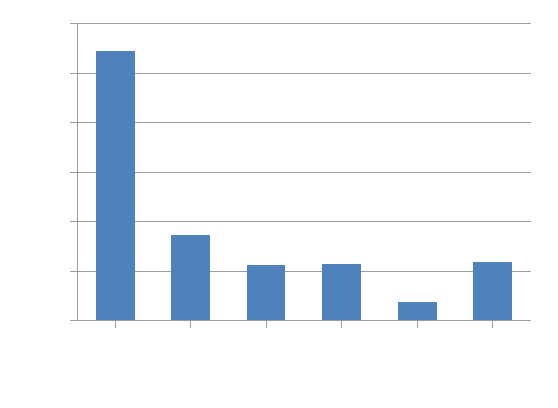
\includegraphics{graph_topology_mcw}}%
    \gplfronttext
  \end{picture}%
\endgroup

%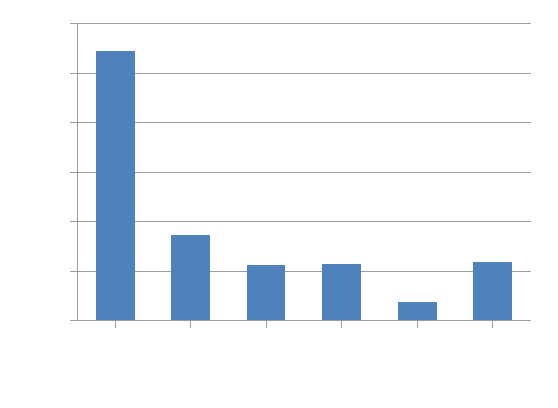
\includegraphics[width=\linewidth]{graph_topology_mcw.eps}
\caption{Minimum channel width achieved by VPR with different hyperedge models and weightings. n is the number of vertices on a hyperedge. TODO JAVEED: Which circuits?}
\label{fig:graph_topology_mcw}
\end{figure}

The star topology with 1/n edge weights achieves the best minimum channel width, confirming that hyperedge cutsize is a good proxy for routability. Consequently, we use this scheme in all future results in this paper. Unlike routability, we found that the post-routing critical path delay was not strongly impacted by the hypergraph conversion scheme used.

\subsubsection{Partitioner Stage Results}\label{sec:partitioner_stage_results}
We compare the performance of the four CAD flow variations described in Section \ref{sec:partitioner_stage} on the 8 largest VTR benchmarks. We again use an unbalance of $5\%$ and split the clustered netlist into two partitions (constraining the packer and/or the placer, as required by the flow under test). The interposer parameters (\% wires cut = $80\%$ and delay increase = 1 ns) and bloat factor ($10\%$ in each dimension) are the same as in Section \ref{sec:hypergraph_to_graph}. Figure \ref{fig:flows_mcw} shows the minimum routable channel width for each partitioning CAD flow variation.

\begin{figure}[!htbp]
\centering
%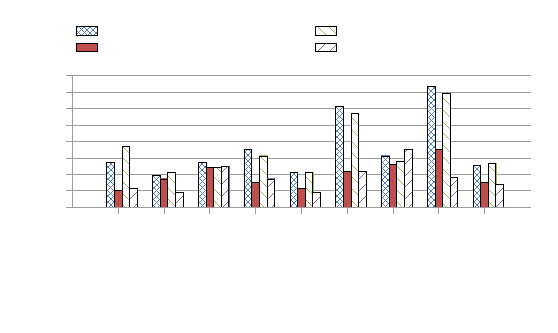
\includegraphics[width=\linewidth]{vpr_flows_mcw.eps}
% GNUPLOT: LaTeX picture with Postscript
\begingroup
  \makeatletter
  \providecommand\color[2][]{%
    \GenericError{(gnuplot) \space\space\space\@spaces}{%
      Package color not loaded in conjunction with
      terminal option `colourtext'%
    }{See the gnuplot documentation for explanation.%
    }{Either use 'blacktext' in gnuplot or load the package
      color.sty in LaTeX.}%
    \renewcommand\color[2][]{}%
  }%
  \providecommand\includegraphics[2][]{%
    \GenericError{(gnuplot) \space\space\space\@spaces}{%
      Package graphicx or graphics not loaded%
    }{See the gnuplot documentation for explanation.%
    }{The gnuplot epslatex terminal needs graphicx.sty or graphics.sty.}%
    \renewcommand\includegraphics[2][]{}%
  }%
  \providecommand\rotatebox[2]{#2}%
  \@ifundefined{ifGPcolor}{%
    \newif\ifGPcolor
    \GPcolortrue
  }{}%
  \@ifundefined{ifGPblacktext}{%
    \newif\ifGPblacktext
    \GPblacktexttrue
  }{}%
  % define a \g@addto@macro without @ in the name:
  \let\gplgaddtomacro\g@addto@macro
  % define empty templates for all commands taking text:
  \gdef\gplbacktext{}%
  \gdef\gplfronttext{}%
  \makeatother
  \ifGPblacktext
    % no textcolor at all
    \def\colorrgb#1{}%
    \def\colorgray#1{}%
  \else
    % gray or color?
    \ifGPcolor
      \def\colorrgb#1{\color[rgb]{#1}}%
      \def\colorgray#1{\color[gray]{#1}}%
      \expandafter\def\csname LTw\endcsname{\color{white}}%
      \expandafter\def\csname LTb\endcsname{\color{black}}%
      \expandafter\def\csname LTa\endcsname{\color{black}}%
      \expandafter\def\csname LT0\endcsname{\color[rgb]{1,0,0}}%
      \expandafter\def\csname LT1\endcsname{\color[rgb]{0,1,0}}%
      \expandafter\def\csname LT2\endcsname{\color[rgb]{0,0,1}}%
      \expandafter\def\csname LT3\endcsname{\color[rgb]{1,0,1}}%
      \expandafter\def\csname LT4\endcsname{\color[rgb]{0,1,1}}%
      \expandafter\def\csname LT5\endcsname{\color[rgb]{1,1,0}}%
      \expandafter\def\csname LT6\endcsname{\color[rgb]{0,0,0}}%
      \expandafter\def\csname LT7\endcsname{\color[rgb]{1,0.3,0}}%
      \expandafter\def\csname LT8\endcsname{\color[rgb]{0.5,0.5,0.5}}%
    \else
      % gray
      \def\colorrgb#1{\color{black}}%
      \def\colorgray#1{\color[gray]{#1}}%
      \expandafter\def\csname LTw\endcsname{\color{white}}%
      \expandafter\def\csname LTb\endcsname{\color{black}}%
      \expandafter\def\csname LTa\endcsname{\color{black}}%
      \expandafter\def\csname LT0\endcsname{\color{black}}%
      \expandafter\def\csname LT1\endcsname{\color{black}}%
      \expandafter\def\csname LT2\endcsname{\color{black}}%
      \expandafter\def\csname LT3\endcsname{\color{black}}%
      \expandafter\def\csname LT4\endcsname{\color{black}}%
      \expandafter\def\csname LT5\endcsname{\color{black}}%
      \expandafter\def\csname LT6\endcsname{\color{black}}%
      \expandafter\def\csname LT7\endcsname{\color{black}}%
      \expandafter\def\csname LT8\endcsname{\color{black}}%
    \fi
  \fi
  \setlength{\unitlength}{0.0500bp}%
  \begin{picture}(5040.00,3600.00)%
    \gplgaddtomacro\gplbacktext{%
      \colorrgb{0.61,0.61,0.61}%
      \put(438,1047){\makebox(0,0)[r]{\strut{}\footnotesize{50}}}%
      \colorrgb{0.61,0.61,0.61}%
      \put(438,1310){\makebox(0,0)[r]{\strut{}\footnotesize{100}}}%
      \colorrgb{0.61,0.61,0.61}%
      \put(438,1574){\makebox(0,0)[r]{\strut{}\footnotesize{150}}}%
      \colorrgb{0.61,0.61,0.61}%
      \put(438,1837){\makebox(0,0)[r]{\strut{}\footnotesize{200}}}%
      \colorrgb{0.61,0.61,0.61}%
      \put(438,2100){\makebox(0,0)[r]{\strut{}\footnotesize{250}}}%
      \colorrgb{0.61,0.61,0.61}%
      \put(438,2363){\makebox(0,0)[r]{\strut{}\footnotesize{300}}}%
      \colorrgb{0.61,0.61,0.61}%
      \put(438,2627){\makebox(0,0)[r]{\strut{}\footnotesize{350}}}%
      \colorrgb{0.61,0.61,0.61}%
      \put(438,2890){\makebox(0,0)[r]{\strut{}\footnotesize{400}}}%
      \colorrgb{0.61,0.61,0.61}%
      \put(438,3153){\makebox(0,0)[r]{\strut{}\footnotesize{450}}}%
      \colorrgb{0.61,0.61,0.61}%
      \put(976,888){\rotatebox{45}{\makebox(0,0)[r]{\strut{}\footnotesize{bgm}}}}%
      \colorrgb{0.61,0.61,0.61}%
      \put(1416,888){\rotatebox{45}{\makebox(0,0)[r]{\strut{}\footnotesize{stereovision0}}}}%
      \colorrgb{0.61,0.61,0.61}%
      \put(1855,888){\rotatebox{45}{\makebox(0,0)[r]{\strut{}\footnotesize{stereovision1}}}}%
      \colorrgb{0.61,0.61,0.61}%
      \put(2295,888){\rotatebox{45}{\makebox(0,0)[r]{\strut{}\footnotesize{LU8PEEng}}}}%
      \colorrgb{0.61,0.61,0.61}%
      \put(2734,888){\rotatebox{45}{\makebox(0,0)[r]{\strut{}\footnotesize{mkDelayWorker32B}}}}%
      \colorrgb{0.61,0.61,0.61}%
      \put(3173,888){\rotatebox{45}{\makebox(0,0)[r]{\strut{}\footnotesize{stereovision2}}}}%
      \colorrgb{0.61,0.61,0.61}%
      \put(3613,888){\rotatebox{45}{\makebox(0,0)[r]{\strut{}\footnotesize{mcml}}}}%
      \colorrgb{0.61,0.61,0.61}%
      \put(4052,888){\rotatebox{45}{\makebox(0,0)[r]{\strut{}\footnotesize{LU32PEEng}}}}%
      \colorrgb{0.61,0.61,0.61}%
      \put(4492,888){\rotatebox{45}{\makebox(0,0)[r]{\strut{}\footnotesize{geomean}}}}%
      \csname LTb\endcsname%
      \put(48,2100){\rotatebox{-270}{\makebox(0,0){\strut{}\footnotesize{\textbf{Minimum Channel Width}}}}}%
      \put(2734,42){\makebox(0,0){\strut{}\footnotesize{\textbf{Circuit}}}}%
    }%
    \gplgaddtomacro\gplfronttext{%
      \csname LTb\endcsname%
      \put(816,3459){\makebox(0,0)[l]{\strut{}\footnotesize{No Partitioning (Base Flow)}}}%
      \csname LTb\endcsname%
      \put(816,3302){\makebox(0,0)[l]{\strut{}\footnotesize{Packing Constraints Only}}}%
      \csname LTb\endcsname%
      \put(3039,3459){\makebox(0,0)[l]{\strut{}\footnotesize{Placement Constraints Only}}}%
      \csname LTb\endcsname%
      \put(3039,3302){\makebox(0,0)[l]{\strut{}\footnotesize{Packing and Placement Constraints}}}%
    }%
    \gplbacktext
    \put(0,0){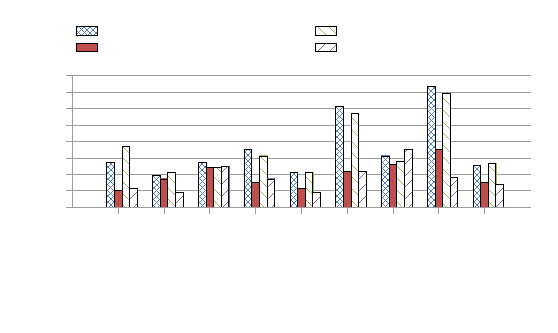
\includegraphics{vpr_flows_mcw}}%
    \gplfronttext
  \end{picture}%
\endgroup

\caption{Minimum channel width achieved by VPR with the different partitioning flows.}
\label{fig:flows_mcw}
\end{figure}

On average, the best minimum channel width was obtained when constraining both packing and placement. However, constraining packing alone performed significantly better than constraining placement alone. This shows that the VPR packer strongly benefits from partitioning constraints when targeting an interposer-based architecture, likely because it forbids the packing of primitives that are not naturally related into one function block. Interestingly, other recent work targeting conventional FPGAs has shown that using a partitioner to guide packing benefits routability\cite{feng2014rent}. On the other hand, The VPR placement algorithm with the enhancements described in Section 4 sees only a modest routability benefit from the partitioning constraints.

For the same set of circuits, we computed the critical path delay at a channel width equal to 1.3x the minimum. The results are shown in Figure \ref{fig:flows_crit_path}.

\begin{figure}[!htbp]
\centering
% GNUPLOT: LaTeX picture with Postscript
\begingroup
  \makeatletter
  \providecommand\color[2][]{%
    \GenericError{(gnuplot) \space\space\space\@spaces}{%
      Package color not loaded in conjunction with
      terminal option `colourtext'%
    }{See the gnuplot documentation for explanation.%
    }{Either use 'blacktext' in gnuplot or load the package
      color.sty in LaTeX.}%
    \renewcommand\color[2][]{}%
  }%
  \providecommand\includegraphics[2][]{%
    \GenericError{(gnuplot) \space\space\space\@spaces}{%
      Package graphicx or graphics not loaded%
    }{See the gnuplot documentation for explanation.%
    }{The gnuplot epslatex terminal needs graphicx.sty or graphics.sty.}%
    \renewcommand\includegraphics[2][]{}%
  }%
  \providecommand\rotatebox[2]{#2}%
  \@ifundefined{ifGPcolor}{%
    \newif\ifGPcolor
    \GPcolortrue
  }{}%
  \@ifundefined{ifGPblacktext}{%
    \newif\ifGPblacktext
    \GPblacktexttrue
  }{}%
  % define a \g@addto@macro without @ in the name:
  \let\gplgaddtomacro\g@addto@macro
  % define empty templates for all commands taking text:
  \gdef\gplbacktext{}%
  \gdef\gplfronttext{}%
  \makeatother
  \ifGPblacktext
    % no textcolor at all
    \def\colorrgb#1{}%
    \def\colorgray#1{}%
  \else
    % gray or color?
    \ifGPcolor
      \def\colorrgb#1{\color[rgb]{#1}}%
      \def\colorgray#1{\color[gray]{#1}}%
      \expandafter\def\csname LTw\endcsname{\color{white}}%
      \expandafter\def\csname LTb\endcsname{\color{black}}%
      \expandafter\def\csname LTa\endcsname{\color{black}}%
      \expandafter\def\csname LT0\endcsname{\color[rgb]{1,0,0}}%
      \expandafter\def\csname LT1\endcsname{\color[rgb]{0,1,0}}%
      \expandafter\def\csname LT2\endcsname{\color[rgb]{0,0,1}}%
      \expandafter\def\csname LT3\endcsname{\color[rgb]{1,0,1}}%
      \expandafter\def\csname LT4\endcsname{\color[rgb]{0,1,1}}%
      \expandafter\def\csname LT5\endcsname{\color[rgb]{1,1,0}}%
      \expandafter\def\csname LT6\endcsname{\color[rgb]{0,0,0}}%
      \expandafter\def\csname LT7\endcsname{\color[rgb]{1,0.3,0}}%
      \expandafter\def\csname LT8\endcsname{\color[rgb]{0.5,0.5,0.5}}%
    \else
      % gray
      \def\colorrgb#1{\color{black}}%
      \def\colorgray#1{\color[gray]{#1}}%
      \expandafter\def\csname LTw\endcsname{\color{white}}%
      \expandafter\def\csname LTb\endcsname{\color{black}}%
      \expandafter\def\csname LTa\endcsname{\color{black}}%
      \expandafter\def\csname LT0\endcsname{\color{black}}%
      \expandafter\def\csname LT1\endcsname{\color{black}}%
      \expandafter\def\csname LT2\endcsname{\color{black}}%
      \expandafter\def\csname LT3\endcsname{\color{black}}%
      \expandafter\def\csname LT4\endcsname{\color{black}}%
      \expandafter\def\csname LT5\endcsname{\color{black}}%
      \expandafter\def\csname LT6\endcsname{\color{black}}%
      \expandafter\def\csname LT7\endcsname{\color{black}}%
      \expandafter\def\csname LT8\endcsname{\color{black}}%
    \fi
  \fi
  \setlength{\unitlength}{0.0500bp}%
  \begin{picture}(5040.00,2880.00)%
    \gplgaddtomacro\gplbacktext{%
      \colorrgb{0.61,0.61,0.61}%
      \put(438,1047){\makebox(0,0)[r]{\strut{}\footnotesize{0}}}%
      \colorrgb{0.61,0.61,0.61}%
      \put(438,1257){\makebox(0,0)[r]{\strut{}\footnotesize{20}}}%
      \colorrgb{0.61,0.61,0.61}%
      \put(438,1468){\makebox(0,0)[r]{\strut{}\footnotesize{40}}}%
      \colorrgb{0.61,0.61,0.61}%
      \put(438,1678){\makebox(0,0)[r]{\strut{}\footnotesize{60}}}%
      \colorrgb{0.61,0.61,0.61}%
      \put(438,1888){\makebox(0,0)[r]{\strut{}\footnotesize{80}}}%
      \colorrgb{0.61,0.61,0.61}%
      \put(438,2099){\makebox(0,0)[r]{\strut{}\footnotesize{100}}}%
      \colorrgb{0.61,0.61,0.61}%
      \put(438,2309){\makebox(0,0)[r]{\strut{}\footnotesize{120}}}%
      \colorrgb{0.61,0.61,0.61}%
      \put(976,888){\rotatebox{45}{\makebox(0,0)[r]{\strut{}\footnotesize{bgm}}}}%
      \colorrgb{0.61,0.61,0.61}%
      \put(1416,888){\rotatebox{45}{\makebox(0,0)[r]{\strut{}\footnotesize{stereovision0}}}}%
      \colorrgb{0.61,0.61,0.61}%
      \put(1855,888){\rotatebox{45}{\makebox(0,0)[r]{\strut{}\footnotesize{stereovision1}}}}%
      \colorrgb{0.61,0.61,0.61}%
      \put(2295,888){\rotatebox{45}{\makebox(0,0)[r]{\strut{}\footnotesize{LU8PEEng}}}}%
      \colorrgb{0.61,0.61,0.61}%
      \put(2734,888){\rotatebox{45}{\makebox(0,0)[r]{\strut{}\footnotesize{mkDelayWorker32B}}}}%
      \colorrgb{0.61,0.61,0.61}%
      \put(3173,888){\rotatebox{45}{\makebox(0,0)[r]{\strut{}\footnotesize{stereovision2}}}}%
      \colorrgb{0.61,0.61,0.61}%
      \put(3613,888){\rotatebox{45}{\makebox(0,0)[r]{\strut{}\footnotesize{mcml}}}}%
      \colorrgb{0.61,0.61,0.61}%
      \put(4052,888){\rotatebox{45}{\makebox(0,0)[r]{\strut{}\footnotesize{LU32PEEng}}}}%
      \colorrgb{0.61,0.61,0.61}%
      \put(4492,888){\rotatebox{45}{\makebox(0,0)[r]{\strut{}\footnotesize{geomean}}}}%
      \csname LTb\endcsname%
      \put(48,1678){\rotatebox{-270}{\makebox(0,0){\strut{}\footnotesize{\textbf{Critical Path Delay (ns)}}}}}%
      \put(2734,42){\makebox(0,0){\strut{}\footnotesize{\textbf{Circuit}}}}%
    }%
    \gplgaddtomacro\gplfronttext{%
      \csname LTb\endcsname%
      \put(816,2739){\makebox(0,0)[l]{\strut{}\footnotesize{No Partitioning (Base Flow)}}}%
      \csname LTb\endcsname%
      \put(816,2582){\makebox(0,0)[l]{\strut{}\footnotesize{Packing Constraints Only}}}%
      \csname LTb\endcsname%
      \put(3111,2739){\makebox(0,0)[l]{\strut{}\footnotesize{Placement Constraints Only}}}%
      \csname LTb\endcsname%
      \put(3111,2582){\makebox(0,0)[l]{\strut{}\footnotesize{Packing and Placement}}}%
      \put(3111,2522){\makebox(0,0)[l]{\strut{}}}%
      \put(3111,2462){\makebox(0,0)[l]{\strut{}\footnotesize{Constraints}}}%
    }%
    \gplbacktext
    \put(0,0){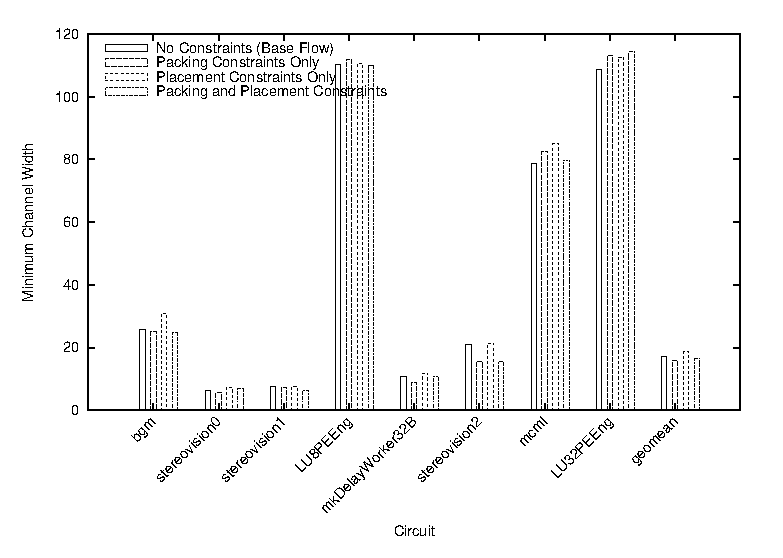
\includegraphics{vpr_flows_crit_path}}%
    \gplfronttext
  \end{picture}%
\endgroup

\caption{Critical path delay achieved by VPR with the different partitioning flows.}
\label{fig:flows_crit_path}
\end{figure}

On average, the critical path delay did not vary significantly between the different partitioning CAD flows, but it appears that partitioning before packing may slightly improve circuit speed, while enforcing these partitioning constraints during placement may slightly reduce circuit speed.

Considering both routability and delay, the best CAD flow constrained both packing and placement with the partitioning result and this is the flow we use in the remainder of this paper.

\subsubsection{\% wires cut}
To see how well the CAD flow works for a range of interposer architectures, we varied the fraction of wires cut and measured the average minimum channel width over the 8 largest VTR circuits. As shown in Figure \ref{fig:wires_cut}, this new flow is a significant improvement over that of [] for FPGAs where more than half the wires are cut at interposer boundaries. It is slightly worse than the traditionally FPGA CAD flow even for an architecture with 0\% of the wires cut, which is a monolithic FPGA, presumably because we have restricted the placer's freedom.

\begin{figure}[!htbp]
\centering
% GNUPLOT: LaTeX picture with Postscript
\begingroup
  \makeatletter
  \providecommand\color[2][]{%
    \GenericError{(gnuplot) \space\space\space\@spaces}{%
      Package color not loaded in conjunction with
      terminal option `colourtext'%
    }{See the gnuplot documentation for explanation.%
    }{Either use 'blacktext' in gnuplot or load the package
      color.sty in LaTeX.}%
    \renewcommand\color[2][]{}%
  }%
  \providecommand\includegraphics[2][]{%
    \GenericError{(gnuplot) \space\space\space\@spaces}{%
      Package graphicx or graphics not loaded%
    }{See the gnuplot documentation for explanation.%
    }{The gnuplot epslatex terminal needs graphicx.sty or graphics.sty.}%
    \renewcommand\includegraphics[2][]{}%
  }%
  \providecommand\rotatebox[2]{#2}%
  \@ifundefined{ifGPcolor}{%
    \newif\ifGPcolor
    \GPcolortrue
  }{}%
  \@ifundefined{ifGPblacktext}{%
    \newif\ifGPblacktext
    \GPblacktexttrue
  }{}%
  % define a \g@addto@macro without @ in the name:
  \let\gplgaddtomacro\g@addto@macro
  % define empty templates for all commands taking text:
  \gdef\gplbacktext{}%
  \gdef\gplfronttext{}%
  \makeatother
  \ifGPblacktext
    % no textcolor at all
    \def\colorrgb#1{}%
    \def\colorgray#1{}%
  \else
    % gray or color?
    \ifGPcolor
      \def\colorrgb#1{\color[rgb]{#1}}%
      \def\colorgray#1{\color[gray]{#1}}%
      \expandafter\def\csname LTw\endcsname{\color{white}}%
      \expandafter\def\csname LTb\endcsname{\color{black}}%
      \expandafter\def\csname LTa\endcsname{\color{black}}%
      \expandafter\def\csname LT0\endcsname{\color[rgb]{1,0,0}}%
      \expandafter\def\csname LT1\endcsname{\color[rgb]{0,1,0}}%
      \expandafter\def\csname LT2\endcsname{\color[rgb]{0,0,1}}%
      \expandafter\def\csname LT3\endcsname{\color[rgb]{1,0,1}}%
      \expandafter\def\csname LT4\endcsname{\color[rgb]{0,1,1}}%
      \expandafter\def\csname LT5\endcsname{\color[rgb]{1,1,0}}%
      \expandafter\def\csname LT6\endcsname{\color[rgb]{0,0,0}}%
      \expandafter\def\csname LT7\endcsname{\color[rgb]{1,0.3,0}}%
      \expandafter\def\csname LT8\endcsname{\color[rgb]{0.5,0.5,0.5}}%
    \else
      % gray
      \def\colorrgb#1{\color{black}}%
      \def\colorgray#1{\color[gray]{#1}}%
      \expandafter\def\csname LTw\endcsname{\color{white}}%
      \expandafter\def\csname LTb\endcsname{\color{black}}%
      \expandafter\def\csname LTa\endcsname{\color{black}}%
      \expandafter\def\csname LT0\endcsname{\color{black}}%
      \expandafter\def\csname LT1\endcsname{\color{black}}%
      \expandafter\def\csname LT2\endcsname{\color{black}}%
      \expandafter\def\csname LT3\endcsname{\color{black}}%
      \expandafter\def\csname LT4\endcsname{\color{black}}%
      \expandafter\def\csname LT5\endcsname{\color{black}}%
      \expandafter\def\csname LT6\endcsname{\color{black}}%
      \expandafter\def\csname LT7\endcsname{\color{black}}%
      \expandafter\def\csname LT8\endcsname{\color{black}}%
    \fi
  \fi
  \setlength{\unitlength}{0.0500bp}%
  \begin{picture}(5040.00,3600.00)%
    \gplgaddtomacro\gplbacktext{%
      \colorrgb{0.61,0.61,0.61}%
      \put(438,375){\makebox(0,0)[r]{\strut{}\footnotesize{100}}}%
      \colorrgb{0.61,0.61,0.61}%
      \put(438,794){\makebox(0,0)[r]{\strut{}\footnotesize{120}}}%
      \colorrgb{0.61,0.61,0.61}%
      \put(438,1214){\makebox(0,0)[r]{\strut{}\footnotesize{140}}}%
      \colorrgb{0.61,0.61,0.61}%
      \put(438,1633){\makebox(0,0)[r]{\strut{}\footnotesize{160}}}%
      \colorrgb{0.61,0.61,0.61}%
      \put(438,2052){\makebox(0,0)[r]{\strut{}\footnotesize{180}}}%
      \colorrgb{0.61,0.61,0.61}%
      \put(438,2471){\makebox(0,0)[r]{\strut{}\footnotesize{200}}}%
      \colorrgb{0.61,0.61,0.61}%
      \put(438,2891){\makebox(0,0)[r]{\strut{}\footnotesize{220}}}%
      \colorrgb{0.61,0.61,0.61}%
      \put(438,3310){\makebox(0,0)[r]{\strut{}\footnotesize{240}}}%
      \colorrgb{0.61,0.61,0.61}%
      \put(537,252){\makebox(0,0){\strut{}\footnotesize{0}}}%
      \colorrgb{0.61,0.61,0.61}%
      \put(1025,252){\makebox(0,0){\strut{}\footnotesize{10}}}%
      \colorrgb{0.61,0.61,0.61}%
      \put(1513,252){\makebox(0,0){\strut{}\footnotesize{20}}}%
      \colorrgb{0.61,0.61,0.61}%
      \put(2002,252){\makebox(0,0){\strut{}\footnotesize{30}}}%
      \colorrgb{0.61,0.61,0.61}%
      \put(2490,252){\makebox(0,0){\strut{}\footnotesize{40}}}%
      \colorrgb{0.61,0.61,0.61}%
      \put(2978,252){\makebox(0,0){\strut{}\footnotesize{50}}}%
      \colorrgb{0.61,0.61,0.61}%
      \put(3466,252){\makebox(0,0){\strut{}\footnotesize{60}}}%
      \colorrgb{0.61,0.61,0.61}%
      \put(3955,252){\makebox(0,0){\strut{}\footnotesize{70}}}%
      \colorrgb{0.61,0.61,0.61}%
      \put(4443,252){\makebox(0,0){\strut{}\footnotesize{80}}}%
      \colorrgb{0.61,0.61,0.61}%
      \put(4931,252){\makebox(0,0){\strut{}\footnotesize{90}}}%
      \csname LTb\endcsname%
      \put(48,1842){\rotatebox{-270}{\makebox(0,0){\strut{}\footnotesize{\textbf{Minimum Channel Width}}}}}%
      \put(2734,42){\makebox(0,0){\strut{}\footnotesize{\textbf{\% wires cut}}}}%
    }%
    \gplgaddtomacro\gplfronttext{%
      \csname LTb\endcsname%
      \put(816,3459){\makebox(0,0)[l]{\strut{}\footnotesize{Best CAD Flow}}}%
      \csname LTb\endcsname%
      \put(3003,3459){\makebox(0,0)[l]{\strut{}\footnotesize{Best CAD Flow in \cite{interposer2014}}}}%
    }%
    \gplbacktext
    \put(0,0){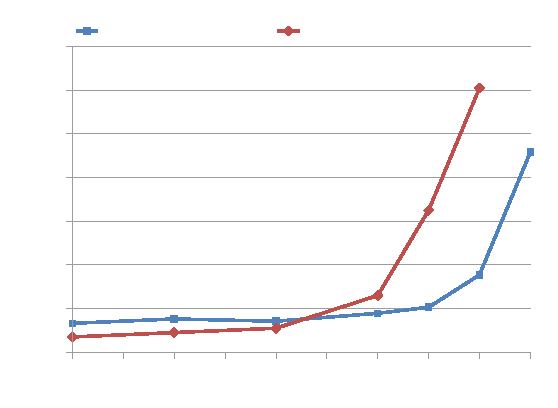
\includegraphics{wires_cut}}%
    \gplfronttext
  \end{picture}%
\endgroup

\caption{Impact of partitioning-based CAD flow on routability for a range of architectures.}
\label{fig:wires_cut}
\end{figure}

\subsubsection{Bloating of the Clustered Netlist due to Partitioning Constraints}
The additional constraints on the packer imposed by partitioning may result in a less dense packing. Figure \ref{fig:packing_bloat} compares the number of complex blocks in the partitioning-constrained and unconstrained clustered netlists.

\begin{figure}[!htbp]
\centering
% GNUPLOT: LaTeX picture with Postscript
\begingroup
  \makeatletter
  \providecommand\color[2][]{%
    \GenericError{(gnuplot) \space\space\space\@spaces}{%
      Package color not loaded in conjunction with
      terminal option `colourtext'%
    }{See the gnuplot documentation for explanation.%
    }{Either use 'blacktext' in gnuplot or load the package
      color.sty in LaTeX.}%
    \renewcommand\color[2][]{}%
  }%
  \providecommand\includegraphics[2][]{%
    \GenericError{(gnuplot) \space\space\space\@spaces}{%
      Package graphicx or graphics not loaded%
    }{See the gnuplot documentation for explanation.%
    }{The gnuplot epslatex terminal needs graphicx.sty or graphics.sty.}%
    \renewcommand\includegraphics[2][]{}%
  }%
  \providecommand\rotatebox[2]{#2}%
  \@ifundefined{ifGPcolor}{%
    \newif\ifGPcolor
    \GPcolortrue
  }{}%
  \@ifundefined{ifGPblacktext}{%
    \newif\ifGPblacktext
    \GPblacktexttrue
  }{}%
  % define a \g@addto@macro without @ in the name:
  \let\gplgaddtomacro\g@addto@macro
  % define empty templates for all commands taking text:
  \gdef\gplbacktext{}%
  \gdef\gplfronttext{}%
  \makeatother
  \ifGPblacktext
    % no textcolor at all
    \def\colorrgb#1{}%
    \def\colorgray#1{}%
  \else
    % gray or color?
    \ifGPcolor
      \def\colorrgb#1{\color[rgb]{#1}}%
      \def\colorgray#1{\color[gray]{#1}}%
      \expandafter\def\csname LTw\endcsname{\color{white}}%
      \expandafter\def\csname LTb\endcsname{\color{black}}%
      \expandafter\def\csname LTa\endcsname{\color{black}}%
      \expandafter\def\csname LT0\endcsname{\color[rgb]{1,0,0}}%
      \expandafter\def\csname LT1\endcsname{\color[rgb]{0,1,0}}%
      \expandafter\def\csname LT2\endcsname{\color[rgb]{0,0,1}}%
      \expandafter\def\csname LT3\endcsname{\color[rgb]{1,0,1}}%
      \expandafter\def\csname LT4\endcsname{\color[rgb]{0,1,1}}%
      \expandafter\def\csname LT5\endcsname{\color[rgb]{1,1,0}}%
      \expandafter\def\csname LT6\endcsname{\color[rgb]{0,0,0}}%
      \expandafter\def\csname LT7\endcsname{\color[rgb]{1,0.3,0}}%
      \expandafter\def\csname LT8\endcsname{\color[rgb]{0.5,0.5,0.5}}%
    \else
      % gray
      \def\colorrgb#1{\color{black}}%
      \def\colorgray#1{\color[gray]{#1}}%
      \expandafter\def\csname LTw\endcsname{\color{white}}%
      \expandafter\def\csname LTb\endcsname{\color{black}}%
      \expandafter\def\csname LTa\endcsname{\color{black}}%
      \expandafter\def\csname LT0\endcsname{\color{black}}%
      \expandafter\def\csname LT1\endcsname{\color{black}}%
      \expandafter\def\csname LT2\endcsname{\color{black}}%
      \expandafter\def\csname LT3\endcsname{\color{black}}%
      \expandafter\def\csname LT4\endcsname{\color{black}}%
      \expandafter\def\csname LT5\endcsname{\color{black}}%
      \expandafter\def\csname LT6\endcsname{\color{black}}%
      \expandafter\def\csname LT7\endcsname{\color{black}}%
      \expandafter\def\csname LT8\endcsname{\color{black}}%
    \fi
  \fi
  \setlength{\unitlength}{0.0500bp}%
  \begin{picture}(5040.00,3600.00)%
    \gplgaddtomacro\gplbacktext{%
      \colorrgb{0.61,0.61,0.61}%
      \put(546,1047){\makebox(0,0)[r]{\strut{}\footnotesize{1000}}}%
      \colorrgb{0.61,0.61,0.61}%
      \put(546,1330){\makebox(0,0)[r]{\strut{}\footnotesize{2000}}}%
      \colorrgb{0.61,0.61,0.61}%
      \put(546,1613){\makebox(0,0)[r]{\strut{}\footnotesize{3000}}}%
      \colorrgb{0.61,0.61,0.61}%
      \put(546,1896){\makebox(0,0)[r]{\strut{}\footnotesize{4000}}}%
      \colorrgb{0.61,0.61,0.61}%
      \put(546,2179){\makebox(0,0)[r]{\strut{}\footnotesize{5000}}}%
      \colorrgb{0.61,0.61,0.61}%
      \put(546,2461){\makebox(0,0)[r]{\strut{}\footnotesize{6000}}}%
      \colorrgb{0.61,0.61,0.61}%
      \put(546,2744){\makebox(0,0)[r]{\strut{}\footnotesize{7000}}}%
      \colorrgb{0.61,0.61,0.61}%
      \put(546,3027){\makebox(0,0)[r]{\strut{}\footnotesize{8000}}}%
      \colorrgb{0.61,0.61,0.61}%
      \put(546,3310){\makebox(0,0)[r]{\strut{}\footnotesize{9000}}}%
      \colorrgb{0.61,0.61,0.61}%
      \put(1121,888){\rotatebox{45}{\makebox(0,0)[r]{\strut{}\footnotesize{bgm}}}}%
      \colorrgb{0.61,0.61,0.61}%
      \put(1597,888){\rotatebox{45}{\makebox(0,0)[r]{\strut{}\footnotesize{stereovision0}}}}%
      \colorrgb{0.61,0.61,0.61}%
      \put(2074,888){\rotatebox{45}{\makebox(0,0)[r]{\strut{}\footnotesize{stereovision1}}}}%
      \colorrgb{0.61,0.61,0.61}%
      \put(2550,888){\rotatebox{45}{\makebox(0,0)[r]{\strut{}\footnotesize{LU8PEEng}}}}%
      \colorrgb{0.61,0.61,0.61}%
      \put(3026,888){\rotatebox{45}{\makebox(0,0)[r]{\strut{}\footnotesize{mkDelayWorker32B}}}}%
      \colorrgb{0.61,0.61,0.61}%
      \put(3502,888){\rotatebox{45}{\makebox(0,0)[r]{\strut{}\footnotesize{stereovision2}}}}%
      \colorrgb{0.61,0.61,0.61}%
      \put(3979,888){\rotatebox{45}{\makebox(0,0)[r]{\strut{}\footnotesize{mcml}}}}%
      \colorrgb{0.61,0.61,0.61}%
      \put(4455,888){\rotatebox{45}{\makebox(0,0)[r]{\strut{}\footnotesize{LU32PEEng}}}}%
      \csname LTb\endcsname%
      \put(48,2178){\rotatebox{-270}{\makebox(0,0){\strut{}\footnotesize{\textbf{Number of Blocks in Clustered Netlist}}}}}%
      \put(2788,42){\makebox(0,0){\strut{}\footnotesize{\textbf{Circuit}}}}%
    }%
    \gplgaddtomacro\gplfronttext{%
      \csname LTb\endcsname%
      \put(924,3459){\makebox(0,0)[l]{\strut{}\footnotesize{No Packing Constraints}}}%
      \csname LTb\endcsname%
      \put(2931,3459){\makebox(0,0)[l]{\strut{}\footnotesize{Packing Constraints}}}%
    }%
    \gplbacktext
    \put(0,0){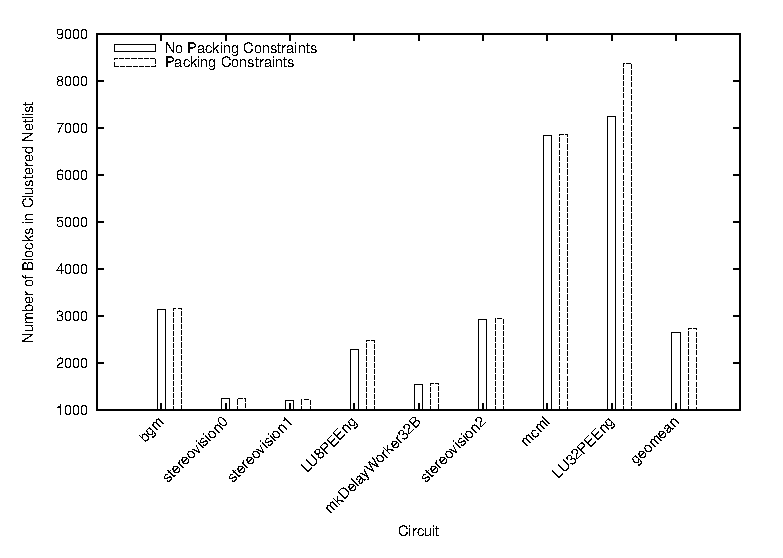
\includegraphics{packing_bloat}}%
    \gplfronttext
  \end{picture}%
\endgroup

\caption{The number of blocks in the clustered netlist with and without partitioning constraints. This is a measure of packing bloat.}
\label{fig:packing_bloat}
\end{figure}

On average, the packing-constrained netlist contained $3.2\%$ more complex blocks than the unconstrained netlist. The LU8PEEng and LU32PEEng circuits were the most affected by this packing bloat. In those circuits, we found that the packing bloat was due almost entirely to poor packing of memory blocks; an interesting area for future work would be to augment the partitioner to understand that some RAM primitives are best kept together in one partition.


%---------------------------------------------------------------
%---------------------------------------------------------------
%---------------------------------------------------------------
\section{Architecture Results}
\label{resultsSection}

Using the best CAD settings found in Section~\ref{cadSection} and the best CAD flow described in Section~\ref{sec:CADflow}, we analyze the impact of the key architecture parameters: \textit{\% wires cut}, \textit{delay increase}, \textit{number of cuts}, and \textit{interposer-routing interface}. We run all the experiments using the setup detailed in Section~\ref{sec:CADeffect}.

%   - routing-interposer interface
\subsection{Routing-Interposer Interface}
As described in \ref{sec:interposer-routing-interface}, we have added three boolean options to VPR that allow us to experiment with different routing-interposer interfaces. Some interface choices provide more flexibility to route signals between different dice and hence help us achieve lower \textit{minimum channel width} and \textit{critical path delay}.

To measure the impact of routing-interposer interface parameters, we set \textit{delay increase}=$1ns$, \textit{number of cuts=1}, and \textit{\% wires cut=80\%}; then, we measure the impact of the \textit{bidirectional interposer wires}, \textit{fanin transfer}, and \textit{fanout transfer} parameters in different combinations. Figure~\ref{fig:all_arch_experiments} summarizes the results of these experiments; all results are normalized to the least flexible routing-interposer interface: one in which 80\% of wires end at the interposer and the other 20\% cross the interposer with the same directionality and routing switches they would have in a conventional FPGA.

\begin{figure}[!h]
\centering
\includegraphics[width=\linewidth]{arch_experiments4.eps}
\caption{Impact of routing-interposer interface flexibility on minimum channel width and circuit speed.}
\label{fig:all_arch_experiments}
\end{figure}

Figure~\ref{fig:all_arch_experiments} shows that using bidirectional interposer wires instead of unidirectional wires (column \textit{b} in Figure~\ref{fig:all_arch_experiments}) improves minimum channel width by 1\% and critical path delay by 0.5\%. Therefore, while it is beneficial to use bidirectional interposer wires, in isolation they do not dramatically improve performance.

Adding multiplexers in front of interposer wires allows dangling routing wires to connect to interposer wires (\textit{``fanin transfer"}) and adding extra load on the output of the interposer wires (\textit{``fanout transfer"}) allows the interposer wire to drive dangling wires on the other side of the cut. Therefore these modifications provide higher flexibility to better utilize interposer wires. Figure~\ref{fig:all_arch_experiments} shows that enabling these two options alone without using bidirectional interposer wires (column \textit{c} in Figure~\ref{fig:all_arch_experiments}) reduces minimum channel width by 3\% and reduces critical path delay by 1\%. 

Moreover, better performance can be achieved if either of these two options is used together with bidirectional interposer wires. Enabling \textit{fanout transfer} with bidirectional interposer wires (column \textit{d} in Figure~\ref{fig:all_arch_experiments}) reduces the minimum channel width by 9\% and critical path delay by 0.7\%. Enabling \textit{fanin transfer} with bidirectional interposer wires (column \textit{e} in Figure~\ref{fig:all_arch_experiments}) has an even stronger impact and reduces the minimum channel width by 10\% and critical path delay by 0.7\%. This signifies that added flexibility to drive an interposer wire is more important for routability than added flexibility allowing an interposer wire to drive multiple vertical routing wires on the other side of the cut.

Enabling all of these architecture modifications simultaneously (column \textit{f} in Figure~\ref{fig:all_arch_experiments}) provides the highest level of flexibility for the router and achieves 11.2\% reduction in minimum channel width and 1.3\% reduction in critical path delay. These models show that interposer-based FPGAs significantly benefit from hardware that provides a flexible routing-interposer interface. It is important both to make the interposer wires easier to access with additional routing switches \textit{and} to make them bidirectional to accommodate asymmetric routing demand.

The \textit{fanin transfer} and \textit{fanout transfer} options ensure that no vertical routing wires are dangling at the cutline; hence, each vertical routing wire either has exactly \textit{one} interposer wire driving it or it drives a mux feeding exactly \textit{one} interposer wire. As a final experiment, we try to add additional fanins and fanouts to interposer wires, so that each vertical routing wire can \textit{potentially} drive multiple interposer wires, or be driven by one of many interposer wires. We found that adding these extra fanouts to interposer wires does not help performance or area, but adding additional fanins to interposer wire muxes helps reduce the minimum channel width while maintaining the same critical path delay. As shown in Figure~\ref{fig:additional_fanins}, adding 4 additional inputs to interposer wire muxes reduces the minimum channel width by 1\% and adding 8 additional inputs reduces minimum channel width by 1.5\%. After that point the performance is no longer limited by the ability to get on an interposer wire and hence we do not see any gains for adding more than 8 additional inputs. Notice that column \textit{0} of Figure~\ref{fig:additional_fanins} is the same as column \textit{f} of Figure~\ref{fig:all_arch_experiments}.

\begin{figure}[!h]
\centering
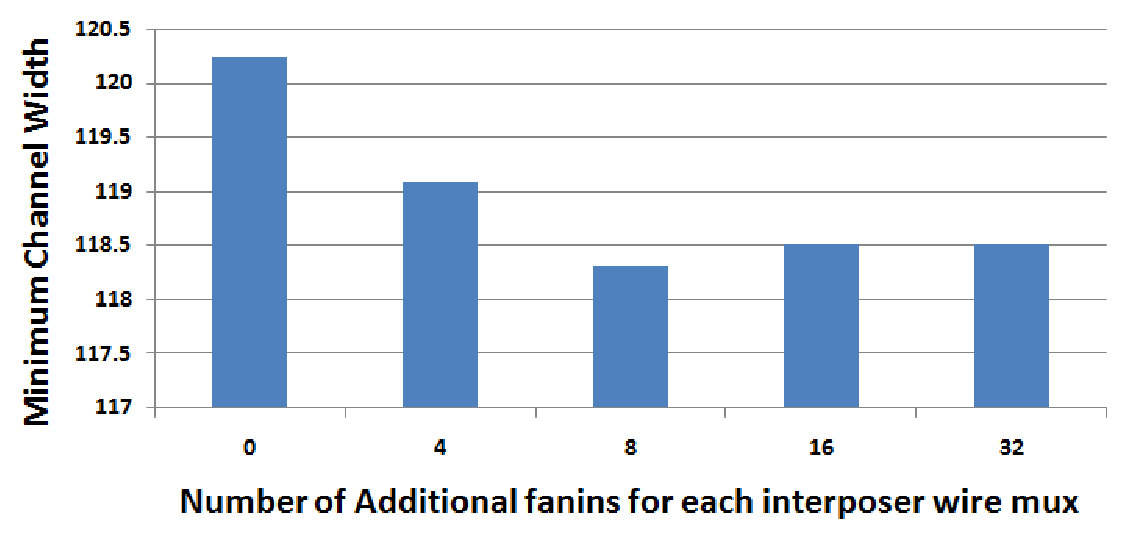
\includegraphics[width=\linewidth]{additional_fanins_2.eps}
\caption{Adding up to 8 extra fanins to interposer wire muxes helps reduce minimum channel width.}
\label{fig:additional_fanins}
\end{figure}

Clearly using bidirectional interposer wires with fanin transfer and fanout transfer is very beneficial, so we use these parameters in all future experiments. Adding additional fanin beyond transferring the fanin of cut wires is only a small further benefit so we use additional fanin=0 in subsequent sections. Adding these additional multiplexers and making the interposer drivers tri-statable causes less than a 0.1\% die area increase as 10,000 muxes per cut would be typical in a large FPGA~\cite{xilinx7series} which is a very small fraction of the several million routing multiplexers in a large FPGA die.


%   - Channel width vs % wires cut
\subsection{Interposer Wiring Capacity (\% wires cut)}
\label{sec:resultsWiringCapacity}

To analyze the impact of the number of cut wires we ran experiments varying only this parameter while leaving the other parameters constant. We use \textit{number of cuts} $= 1$ (i.e. two dice), \textit{increased delay} $= 1ns$, \textit{bidirectional interposer wires = on}, \textit{fanin transfer = on}, and \textit{fanout transfer = on}.

Figure~\ref{fig:standard_minW} shows the graph of minimum channel width versus \textit{\% wires cut}. It can be noted from this graph that the minimum channel width is essentially constant up to 60\% of wires cut, indicating that the CAD flow is able to avoid saturating the interposer routing until that point. When more than 80\% of the wires are cut however (i.e. the interposer provides less than 20\% of the usual within-die routing capacity), the minimum channel width grows rapidly, indicating that the interposer routing bandwidth has become a limiting factor.

\begin{figure}[!htbp]
\centering
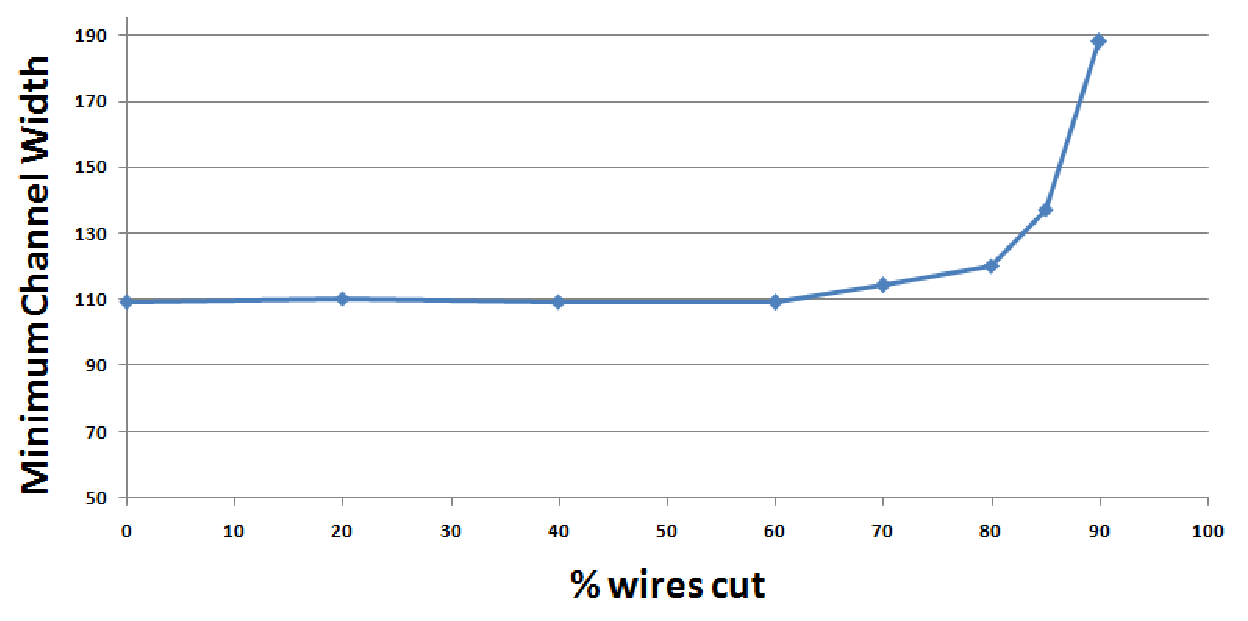
\includegraphics[width=\linewidth]{MinChW_3.eps}
\caption{Minimum channel width vs. \textit{\% wires cut} for 2 dice and $1ns$ of \textit{delay increase}.}
\label{fig:standard_minW}
\end{figure}

Figure \ref{fig:crossingwires} provides an alternative way to visualize the relationship between interposer routing supply and routability. This figure shows how the geometric average minimum channel width required within the FPGA dice varies as the geometric average of the \emph{absolute} number of wires crossing the interposer in each channel varies, again for 2-die system. When 110 tracks cross the interposer, the interposer channels have the same capacity as the vertical routing channels within each FPGA die. As fewer wires cross the interposer, the channel width required within the FPGA dice increases to compensate for the routing difficulty in crossing the interposer. The increase is gradual as the interposer routing is reduced from 110 tracks per channel to 34 tracks per channel; over this range the routing per channel required in the FPGA dice increases from 110 tracks per channel to 114 tracks per channel. As the routing crossing the interposer is further reduced however, it becomes very difficult to increase the within-die routing sufficiently to compensate. At 18 tracks crossing the interposer channels, for example, the within-die routing must have a channel width of \emph{188} tracks to successfully route the designs. Clearly the CAD tools have the ability to trade-off interposer routing for within-die routing over a reasonable range but below a certain level (20\% of the original within-die minimum channel width in our experiments) routability becomes almost solely limited by the wiring crossing the interposer and further reduction in interposer routing is not productive.

\begin{figure}[!t]
\centering
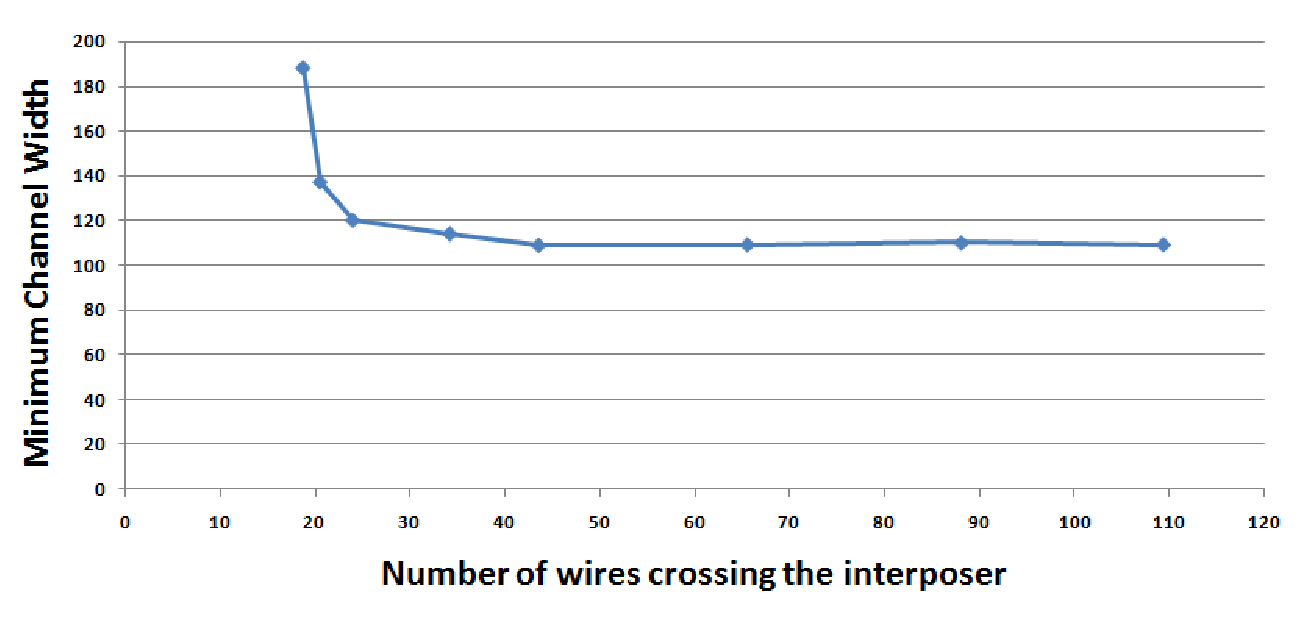
\includegraphics[width=\linewidth]{numberofcrossingwires_new_2.eps}
\caption{Geometric mean of required intra-die minimum channel width vs. geometric mean of the number of wires crossing the interposer for 2 dice and $1ns$ of \textit{delay increase}.}
\label{fig:crossingwires}
\end{figure}

The critical path delay, depicted in Figure~\ref{fig:delays_crit}, on the other hand, is not strongly influenced by the percentage of wires cut, as the critical path delay at 80\% of the wires cut is essentially the same as at 0\% wires cut. Note, however, that this same critical path delay is achieved at a much higher channel width when \textit{\% wires cut} is greater than 80\%.

%   - Delay vs % wires cut & wire delay
\subsection{Circuit Speed vs. Interposer Delay}

\begin{figure}[!b]
\centering
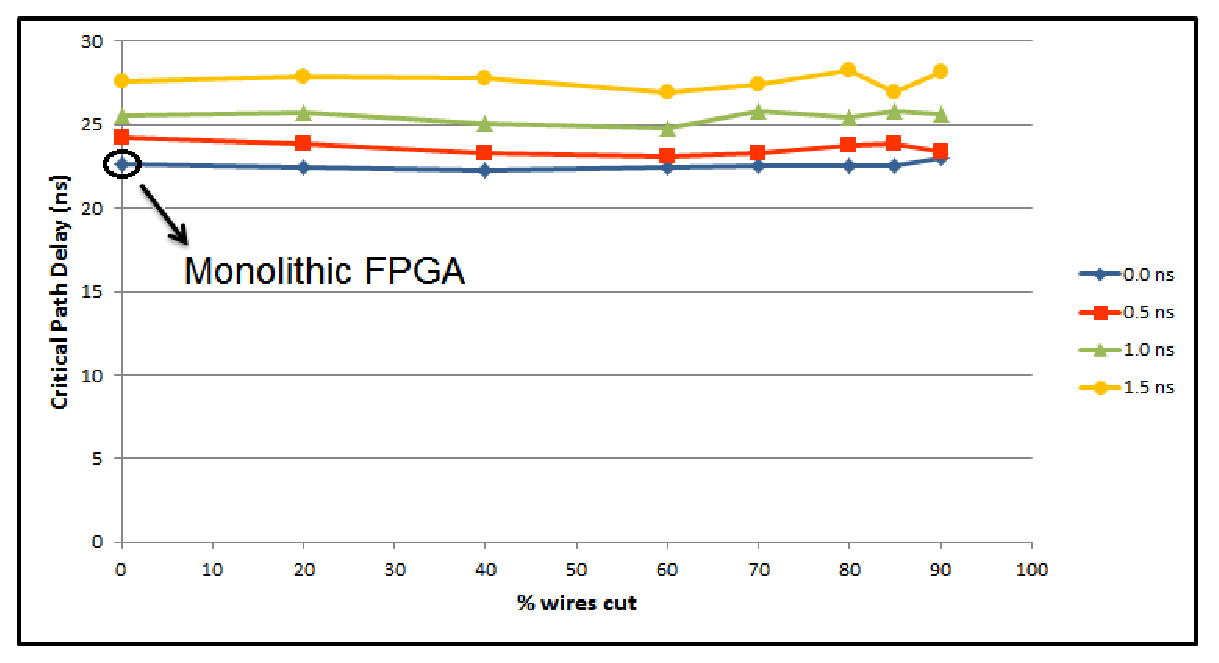
\includegraphics[width=\linewidth]{delays_crit_path_new.eps}
\caption{Critical path delay vs. \textit{\% wires cut} for 2 dice and $0.0$, $0.5$, $1.0$ and $1.5ns$ of \textit{delay increase}.}
\label{fig:delays_crit}
\end{figure}

To investigate the impact of the interposer delay (\textit{delay increase}), we keep all other interposer parameters constant and sweep the \textit{delay increase} from 0 to 1.5 \textit{ns}. We use \textit{number of cuts} $= 1$ (i.e. two dice), \textit{bidirectional interposer wires = on}, \textit{fanin transfer = on}, and \textit{fanout transfer = on}.

Figure \ref{fig:delays_crit} shows critical path delay versus \textit{\% wires cut} for 4 different values of \textit{delay increase}. The penalty in critical path delay is significant, ranging between $1$ and $3.7$ times the interposer \textit{delay increase}, when compared to the case where the interposer adds no delay. Note that the 0\% wires cut with a 0 ns \textit{delay increase} in Figure \ref{fig:delays_crit} corresponds to a traditional monolithic FPGA. The speed of an interposer-based FPGA is strongly correlated to \textit{delay increase}: a $0.5ns$ interposer delay increases the critical path delay by 4\%, while a $1ns$ interposer delay increases critical path delay by approximately 12\% vs. a monolithic FPGA. But once again, the critical path delay shows little correlation to the \textit{\% wires cut}.

%   - Impact of # of cutlines
\subsection{Impact of Number of Dice}
\label{num_dice_impact}
To examine the impact of the number of dice used to construct an interposer-based FPGA, we compare the minimum channel width for FPGA systems composed of four dice and two dice, respectively, while varying the fraction of wires cut at the interposer boundaries. We used the best CAD flow from Section \ref{sec:partitioner_stage_results} and the same interposer routing architecture parameters as Section \ref{sec:resultsWiringCapacity}. 
As Figure \ref{fig:wires_cut_4part} shows, four-die systems perform almost as well in routability as two-die systems until the \textit{\% wires cut} exceeds 80\%, at which point routability is worse for the four-die system. 

\begin{figure}[!htbp]
\centering
% GNUPLOT: LaTeX picture with Postscript
\begingroup
  \makeatletter
  \providecommand\color[2][]{%
    \GenericError{(gnuplot) \space\space\space\@spaces}{%
      Package color not loaded in conjunction with
      terminal option `colourtext'%
    }{See the gnuplot documentation for explanation.%
    }{Either use 'blacktext' in gnuplot or load the package
      color.sty in LaTeX.}%
    \renewcommand\color[2][]{}%
  }%
  \providecommand\includegraphics[2][]{%
    \GenericError{(gnuplot) \space\space\space\@spaces}{%
      Package graphicx or graphics not loaded%
    }{See the gnuplot documentation for explanation.%
    }{The gnuplot epslatex terminal needs graphicx.sty or graphics.sty.}%
    \renewcommand\includegraphics[2][]{}%
  }%
  \providecommand\rotatebox[2]{#2}%
  \@ifundefined{ifGPcolor}{%
    \newif\ifGPcolor
    \GPcolortrue
  }{}%
  \@ifundefined{ifGPblacktext}{%
    \newif\ifGPblacktext
    \GPblacktexttrue
  }{}%
  % define a \g@addto@macro without @ in the name:
  \let\gplgaddtomacro\g@addto@macro
  % define empty templates for all commands taking text:
  \gdef\gplbacktext{}%
  \gdef\gplfronttext{}%
  \makeatother
  \ifGPblacktext
    % no textcolor at all
    \def\colorrgb#1{}%
    \def\colorgray#1{}%
  \else
    % gray or color?
    \ifGPcolor
      \def\colorrgb#1{\color[rgb]{#1}}%
      \def\colorgray#1{\color[gray]{#1}}%
      \expandafter\def\csname LTw\endcsname{\color{white}}%
      \expandafter\def\csname LTb\endcsname{\color{black}}%
      \expandafter\def\csname LTa\endcsname{\color{black}}%
      \expandafter\def\csname LT0\endcsname{\color[rgb]{1,0,0}}%
      \expandafter\def\csname LT1\endcsname{\color[rgb]{0,1,0}}%
      \expandafter\def\csname LT2\endcsname{\color[rgb]{0,0,1}}%
      \expandafter\def\csname LT3\endcsname{\color[rgb]{1,0,1}}%
      \expandafter\def\csname LT4\endcsname{\color[rgb]{0,1,1}}%
      \expandafter\def\csname LT5\endcsname{\color[rgb]{1,1,0}}%
      \expandafter\def\csname LT6\endcsname{\color[rgb]{0,0,0}}%
      \expandafter\def\csname LT7\endcsname{\color[rgb]{1,0.3,0}}%
      \expandafter\def\csname LT8\endcsname{\color[rgb]{0.5,0.5,0.5}}%
    \else
      % gray
      \def\colorrgb#1{\color{black}}%
      \def\colorgray#1{\color[gray]{#1}}%
      \expandafter\def\csname LTw\endcsname{\color{white}}%
      \expandafter\def\csname LTb\endcsname{\color{black}}%
      \expandafter\def\csname LTa\endcsname{\color{black}}%
      \expandafter\def\csname LT0\endcsname{\color{black}}%
      \expandafter\def\csname LT1\endcsname{\color{black}}%
      \expandafter\def\csname LT2\endcsname{\color{black}}%
      \expandafter\def\csname LT3\endcsname{\color{black}}%
      \expandafter\def\csname LT4\endcsname{\color{black}}%
      \expandafter\def\csname LT5\endcsname{\color{black}}%
      \expandafter\def\csname LT6\endcsname{\color{black}}%
      \expandafter\def\csname LT7\endcsname{\color{black}}%
      \expandafter\def\csname LT8\endcsname{\color{black}}%
    \fi
  \fi
  \setlength{\unitlength}{0.0500bp}%
  \begin{picture}(5040.00,2160.00)%
    \gplgaddtomacro\gplbacktext{%
      \colorrgb{0.61,0.61,0.61}%
      \put(438,375){\makebox(0,0)[r]{\strut{}\footnotesize{100}}}%
      \colorrgb{0.61,0.61,0.61}%
      \put(438,541){\makebox(0,0)[r]{\strut{}\footnotesize{110}}}%
      \colorrgb{0.61,0.61,0.61}%
      \put(438,707){\makebox(0,0)[r]{\strut{}\footnotesize{120}}}%
      \colorrgb{0.61,0.61,0.61}%
      \put(438,873){\makebox(0,0)[r]{\strut{}\footnotesize{130}}}%
      \colorrgb{0.61,0.61,0.61}%
      \put(438,1039){\makebox(0,0)[r]{\strut{}\footnotesize{140}}}%
      \colorrgb{0.61,0.61,0.61}%
      \put(438,1206){\makebox(0,0)[r]{\strut{}\footnotesize{150}}}%
      \colorrgb{0.61,0.61,0.61}%
      \put(438,1372){\makebox(0,0)[r]{\strut{}\footnotesize{160}}}%
      \colorrgb{0.61,0.61,0.61}%
      \put(438,1538){\makebox(0,0)[r]{\strut{}\footnotesize{170}}}%
      \colorrgb{0.61,0.61,0.61}%
      \put(438,1704){\makebox(0,0)[r]{\strut{}\footnotesize{180}}}%
      \colorrgb{0.61,0.61,0.61}%
      \put(438,1870){\makebox(0,0)[r]{\strut{}\footnotesize{190}}}%
      \colorrgb{0.61,0.61,0.61}%
      \put(537,252){\makebox(0,0){\strut{}\footnotesize{0}}}%
      \colorrgb{0.61,0.61,0.61}%
      \put(1025,252){\makebox(0,0){\strut{}\footnotesize{10}}}%
      \colorrgb{0.61,0.61,0.61}%
      \put(1513,252){\makebox(0,0){\strut{}\footnotesize{20}}}%
      \colorrgb{0.61,0.61,0.61}%
      \put(2002,252){\makebox(0,0){\strut{}\footnotesize{30}}}%
      \colorrgb{0.61,0.61,0.61}%
      \put(2490,252){\makebox(0,0){\strut{}\footnotesize{40}}}%
      \colorrgb{0.61,0.61,0.61}%
      \put(2978,252){\makebox(0,0){\strut{}\footnotesize{50}}}%
      \colorrgb{0.61,0.61,0.61}%
      \put(3466,252){\makebox(0,0){\strut{}\footnotesize{60}}}%
      \colorrgb{0.61,0.61,0.61}%
      \put(3955,252){\makebox(0,0){\strut{}\footnotesize{70}}}%
      \colorrgb{0.61,0.61,0.61}%
      \put(4443,252){\makebox(0,0){\strut{}\footnotesize{80}}}%
      \colorrgb{0.61,0.61,0.61}%
      \put(4931,252){\makebox(0,0){\strut{}\footnotesize{90}}}%
      \csname LTb\endcsname%
      \put(48,1122){\rotatebox{-270}{\makebox(0,0){\strut{}\footnotesize{\textbf{Minimum Channel Width}}}}}%
      \put(2734,42){\makebox(0,0){\strut{}\footnotesize{\textbf{\% wires cut}}}}%
    }%
    \gplgaddtomacro\gplfronttext{%
      \csname LTb\endcsname%
      \put(816,2019){\makebox(0,0)[l]{\strut{}\footnotesize{2 Partitions}}}%
      \csname LTb\endcsname%
      \put(2283,2019){\makebox(0,0)[l]{\strut{}\footnotesize{4 Partitions}}}%
    }%
    \gplbacktext
    \put(0,0){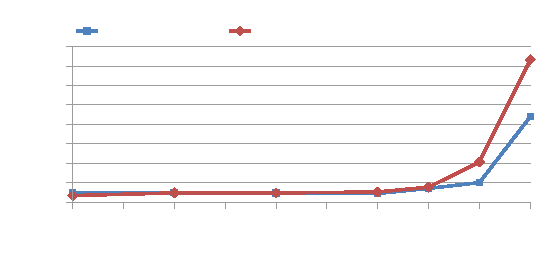
\includegraphics{wires_cut_4part}}%
    \gplfronttext
  \end{picture}%
\endgroup

\caption{Impact of number of dice on routability.}
\label{fig:wires_cut_4part}
\end{figure}

As shown in \ref{fig:crit_path_4part}, systems with more dice are slower; on average the critical path delay is 40\% higher for a four-die system than a two-die system. This speed difference is not significantly affected by the \textit{\% wires cut}. This suggests that the main cause of the slowdown is due to interposer crossings, rather than wire congestion.
\begin{figure}[!htbp]
\centering
% GNUPLOT: LaTeX picture with Postscript
\begingroup
  \makeatletter
  \providecommand\color[2][]{%
    \GenericError{(gnuplot) \space\space\space\@spaces}{%
      Package color not loaded in conjunction with
      terminal option `colourtext'%
    }{See the gnuplot documentation for explanation.%
    }{Either use 'blacktext' in gnuplot or load the package
      color.sty in LaTeX.}%
    \renewcommand\color[2][]{}%
  }%
  \providecommand\includegraphics[2][]{%
    \GenericError{(gnuplot) \space\space\space\@spaces}{%
      Package graphicx or graphics not loaded%
    }{See the gnuplot documentation for explanation.%
    }{The gnuplot epslatex terminal needs graphicx.sty or graphics.sty.}%
    \renewcommand\includegraphics[2][]{}%
  }%
  \providecommand\rotatebox[2]{#2}%
  \@ifundefined{ifGPcolor}{%
    \newif\ifGPcolor
    \GPcolortrue
  }{}%
  \@ifundefined{ifGPblacktext}{%
    \newif\ifGPblacktext
    \GPblacktexttrue
  }{}%
  % define a \g@addto@macro without @ in the name:
  \let\gplgaddtomacro\g@addto@macro
  % define empty templates for all commands taking text:
  \gdef\gplbacktext{}%
  \gdef\gplfronttext{}%
  \makeatother
  \ifGPblacktext
    % no textcolor at all
    \def\colorrgb#1{}%
    \def\colorgray#1{}%
  \else
    % gray or color?
    \ifGPcolor
      \def\colorrgb#1{\color[rgb]{#1}}%
      \def\colorgray#1{\color[gray]{#1}}%
      \expandafter\def\csname LTw\endcsname{\color{white}}%
      \expandafter\def\csname LTb\endcsname{\color{black}}%
      \expandafter\def\csname LTa\endcsname{\color{black}}%
      \expandafter\def\csname LT0\endcsname{\color[rgb]{1,0,0}}%
      \expandafter\def\csname LT1\endcsname{\color[rgb]{0,1,0}}%
      \expandafter\def\csname LT2\endcsname{\color[rgb]{0,0,1}}%
      \expandafter\def\csname LT3\endcsname{\color[rgb]{1,0,1}}%
      \expandafter\def\csname LT4\endcsname{\color[rgb]{0,1,1}}%
      \expandafter\def\csname LT5\endcsname{\color[rgb]{1,1,0}}%
      \expandafter\def\csname LT6\endcsname{\color[rgb]{0,0,0}}%
      \expandafter\def\csname LT7\endcsname{\color[rgb]{1,0.3,0}}%
      \expandafter\def\csname LT8\endcsname{\color[rgb]{0.5,0.5,0.5}}%
    \else
      % gray
      \def\colorrgb#1{\color{black}}%
      \def\colorgray#1{\color[gray]{#1}}%
      \expandafter\def\csname LTw\endcsname{\color{white}}%
      \expandafter\def\csname LTb\endcsname{\color{black}}%
      \expandafter\def\csname LTa\endcsname{\color{black}}%
      \expandafter\def\csname LT0\endcsname{\color{black}}%
      \expandafter\def\csname LT1\endcsname{\color{black}}%
      \expandafter\def\csname LT2\endcsname{\color{black}}%
      \expandafter\def\csname LT3\endcsname{\color{black}}%
      \expandafter\def\csname LT4\endcsname{\color{black}}%
      \expandafter\def\csname LT5\endcsname{\color{black}}%
      \expandafter\def\csname LT6\endcsname{\color{black}}%
      \expandafter\def\csname LT7\endcsname{\color{black}}%
      \expandafter\def\csname LT8\endcsname{\color{black}}%
    \fi
  \fi
  \setlength{\unitlength}{0.0500bp}%
  \begin{picture}(5040.00,3600.00)%
    \gplgaddtomacro\gplbacktext{%
      \colorrgb{0.61,0.61,0.61}%
      \put(402,375){\makebox(0,0)[r]{\strut{}\footnotesize{24}}}%
      \colorrgb{0.61,0.61,0.61}%
      \put(402,864){\makebox(0,0)[r]{\strut{}\footnotesize{26}}}%
      \colorrgb{0.61,0.61,0.61}%
      \put(402,1353){\makebox(0,0)[r]{\strut{}\footnotesize{28}}}%
      \colorrgb{0.61,0.61,0.61}%
      \put(402,1843){\makebox(0,0)[r]{\strut{}\footnotesize{30}}}%
      \colorrgb{0.61,0.61,0.61}%
      \put(402,2332){\makebox(0,0)[r]{\strut{}\footnotesize{32}}}%
      \colorrgb{0.61,0.61,0.61}%
      \put(402,2821){\makebox(0,0)[r]{\strut{}\footnotesize{34}}}%
      \colorrgb{0.61,0.61,0.61}%
      \put(402,3310){\makebox(0,0)[r]{\strut{}\footnotesize{36}}}%
      \colorrgb{0.61,0.61,0.61}%
      \put(501,252){\makebox(0,0){\strut{}\footnotesize{0}}}%
      \colorrgb{0.61,0.61,0.61}%
      \put(993,252){\makebox(0,0){\strut{}\footnotesize{10}}}%
      \colorrgb{0.61,0.61,0.61}%
      \put(1485,252){\makebox(0,0){\strut{}\footnotesize{20}}}%
      \colorrgb{0.61,0.61,0.61}%
      \put(1978,252){\makebox(0,0){\strut{}\footnotesize{30}}}%
      \colorrgb{0.61,0.61,0.61}%
      \put(2470,252){\makebox(0,0){\strut{}\footnotesize{40}}}%
      \colorrgb{0.61,0.61,0.61}%
      \put(2962,252){\makebox(0,0){\strut{}\footnotesize{50}}}%
      \colorrgb{0.61,0.61,0.61}%
      \put(3454,252){\makebox(0,0){\strut{}\footnotesize{60}}}%
      \colorrgb{0.61,0.61,0.61}%
      \put(3947,252){\makebox(0,0){\strut{}\footnotesize{70}}}%
      \colorrgb{0.61,0.61,0.61}%
      \put(4439,252){\makebox(0,0){\strut{}\footnotesize{80}}}%
      \colorrgb{0.61,0.61,0.61}%
      \put(4931,252){\makebox(0,0){\strut{}\footnotesize{90}}}%
      \csname LTb\endcsname%
      \put(48,1842){\rotatebox{-270}{\makebox(0,0){\strut{}\footnotesize{\textbf{Critical Path Delay}}}}}%
      \put(2716,42){\makebox(0,0){\strut{}\footnotesize{\textbf{\% wires cut}}}}%
    }%
    \gplgaddtomacro\gplfronttext{%
      \csname LTb\endcsname%
      \put(780,3459){\makebox(0,0)[l]{\strut{}\footnotesize{2 Partitions}}}%
      \csname LTb\endcsname%
      \put(2247,3459){\makebox(0,0)[l]{\strut{}\footnotesize{4 Partitions}}}%
    }%
    \gplbacktext
    \put(0,0){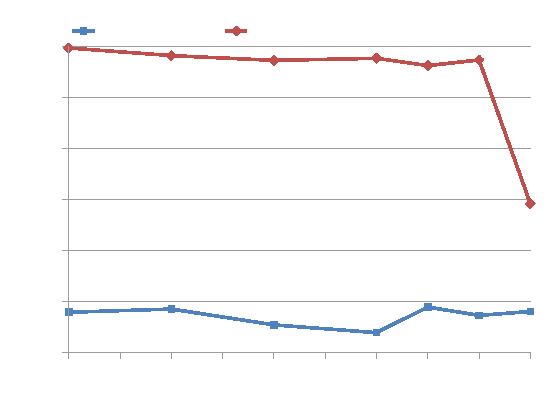
\includegraphics{crit_path_4part}}%
    \gplfronttext
  \end{picture}%
\endgroup

\caption{Impact of number of dice on critical path delay.}
\label{fig:crit_path_4part}
\end{figure}

%   - Impact of aspect ratio
\subsection{Impact of Aspect Ratio}
\label{aspect_ratio_impact}
It is easier to manufacture silicon dice that have an aspect ratio near 1 (i.e. square). Commercial FPGAs are laid out with identical columns, and hence combine multiple identical FPGA dice in \textit{one dimension} on an interposer \cite{xilinxTSV}. As Figure~\ref{fig:square_tall} shows, we can make \textit{either} the FPGA dice square, or the interposer square, but not both. Table \ref{table:squares} compares the routability of these two options for the four-die case. We used the best CAD flow from Section \ref{sec:partitioner_stage_results} and the same routing architecture parameters as Section \ref{sec:resultsWiringCapacity}. 

\begin{figure}[!htbp]
\centering
\subfigure[]{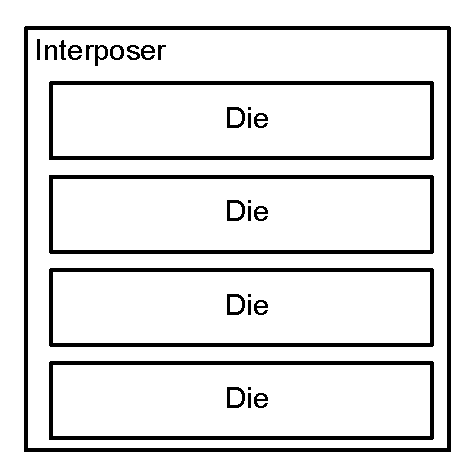
\includegraphics[height = 2.3cm]{square_fpga.pdf}}
\subfigure[]{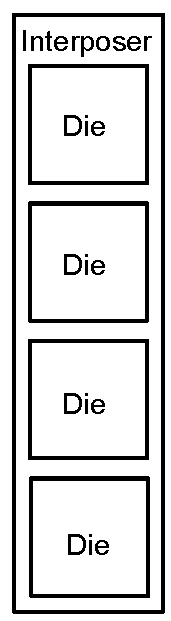
\includegraphics[height = 3.6cm]{tall_fpga.pdf}}
\caption{Devices with (a) a square interposer and (b) square dice.}
\label{fig:square_tall}
\end{figure}

\begin{table}[!htbp]
\centering
\caption{Square interposer and square dice minimum channel widths}
\begin{tabular}{|l|r|r|}
\hline
 & Square Interposer & Square Dice \\ \hline \hline
bgm & 102 & 306 \\ \hline
stereovision0 & 86 & 256 \\ \hline
stereovision1 & 166 & 256 \\ \hline
LU8PEEng & 156 & 126 \\ \hline
mkDelayWorker32B & 96 & 194 \\ \hline
mcml & 196 & 496 \\ \hline
LU32PEEng & 256 & 264 \\ \hhline{|=|=|=|}
geomean & 141 & 252 \\ \hline
\end{tabular}
\label{table:squares}
\end{table}

Compared to square dice, a square interposer (composed of rectangular FPGA dice) results in cutlines that are closer together, and hence more logic blocks are near a cutline. On the other hand, a square interposer has more vertical routing channels, giving it a higher absolute number of wires between FPGA dice. The second effect is the more important one, leading to much better routability for a square interposer than for square dice.

%---------------------------------------------------------------
%---------------------------------------------------------------
%---------------------------------------------------------------
\section{Conclusion}
\label{conclusionSection}
We have extended VPR to target interposer-based multi-FPGA systems. We found that by modifying VPR's placement cost function we can improve routability, while simultaneously improving speed. Modifications to the VPR router lookahead function are crucial to keep compile time reasonable and yield a 31$\times$ speed-up. Incorporating partitioning into the CAD flow is very beneficial. Our best partitioning flow converts nets (hyperedges) to a star graph model, uses Metis to partition the resulting circuit graph, and forces VPR's packer to respect the Metis partitioning to FPGA dice. Taken together, these CAD changes reduce the signal wires that must cross the interposer by an average of 47\% while simultaneously improving circuit speed by 13\% for realistic interposer architectures.

We defined four key architecture parameters for interposer-based FPGAs, and used this extended VPR to analyze their impact on minimum channel width and critical path delay. We find that adding a moderate amount of switching flexibility at the FPGA - interposer boundary has negligible area cost but reduces the required minimum channel width by 13\%. We also find that the multi-die system has good routability so long as the interposer provides sufficient routing bandwidth, and this routing bandwidth can be much less than one would find in a monolithic FPGA. Specifically, if the interposer provides 40\% or more of the channel width required by the monolithic FPGA (an average of 45 wires per channel across our benchmark suite) the routability of the interposer-based FPGA is equivalent to that of a monolithic one. As the interposer signal bandwidth becomes more constrained, routability is impacted but even an interposer providing only 20\% of the monolithic FPGA routing channel bandwidth (22 wires in our experiments) only needs a 10\% increase in the within-FPGA-die routing channel width to compensate.

The \textit{critical path delay} is not strongly influenced by the \textit{\% wires cut} but is strongly influenced by the interposer delay and the number of cuts. On average we find that a 1 ns interposer delay causes an 11\% delay increase in a two-die system vs. a monolithic FPGA. Increasing the number of dice in an interposer-based FPGA only moderately impacts the \textit{minimum channel width}, but does lead to a larger \textit{critical path delay}. The aspect ratio of the interposer-based FPGA is an important architectural parameter; a square interposer containing rectangular FPGA dice has the best routability.

Overall we find the results for interposer-based FPGAs to be very positive. While an interposer can only provide a fraction of the signal count between dice that one would have within a die, the system still has excellent routability so long as the interposer signal count is not pushed to very low values; below 20\% of the within-die routing in our experiments. We have also found that modifications to the CAD flow and routing architecture to exploit interposer-based FPGAs have been very productive. As this is a new area, we believe more routability and timing enhancements can be achieved with further research; for example, a timing-driven partitioner may reduce the delay impact of the interposer.

% use section* for acknowledgement
\section*{Acknowledgment}
This work was supported by Brazil's Ci\^{e}ncia sem Fronteiras scholarship and the NSERC/Altera Industrial Research Chair in Programmable Silicon. Some computations were performed on the GPC supercomputer at the SciNet HPC Consortium.

\bibliographystyle{IEEEtran}
% argument is your BibTeX string definitions and bibliography database(s)
\bibliography{IEEEabrv,./fpga2014paper}

% ----- BIOGRAPHY ------------------
% \vspace{-2in}
\vfill
\begin{IEEEbiography}[{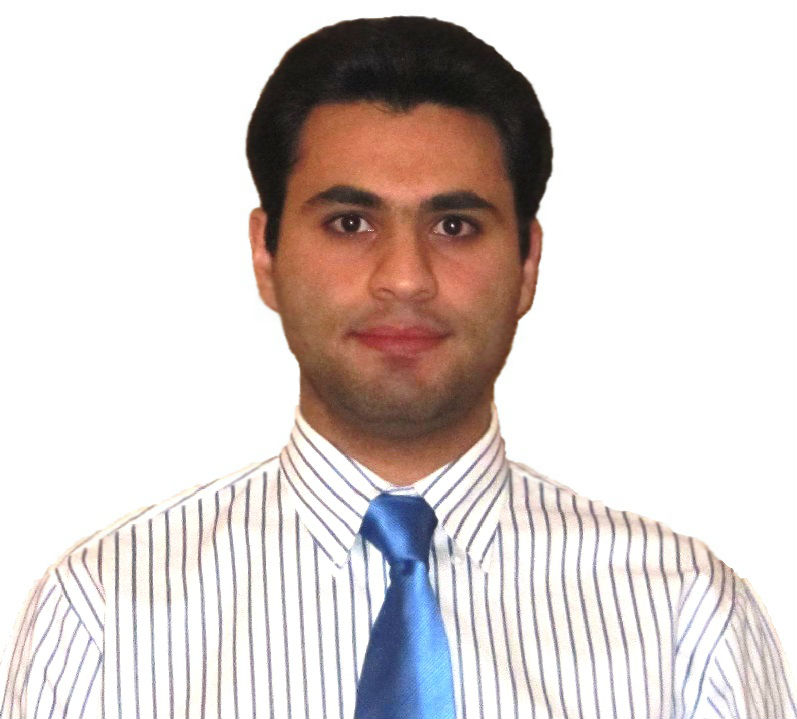
\includegraphics[width=1in,height=1.25in,clip,keepaspectratio]{enasiri}}]{Ehsan Nasiri} received the Bachelor of Applied Science in Computer Engineering from the University of Toronto in 2012, and the M.Eng. degree in ECE from the University of Toronto in 2015. He has been a Software Engineer at Altera since 2012.
\end{IEEEbiography}

\begin{IEEEbiography}[{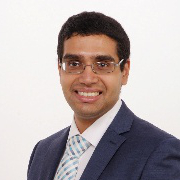
\includegraphics[width=1in,height=1.25in,clip,keepaspectratio]{javeed}}]{Javeed Shaikh} received the BEng degree in Electrical Engineering from McGill University in 2011 and the MEng degree in ECE from the University of Toronto in 2014. He has been a Software Engineer at Google since 2013.
\end{IEEEbiography}

\begin{IEEEbiography}[{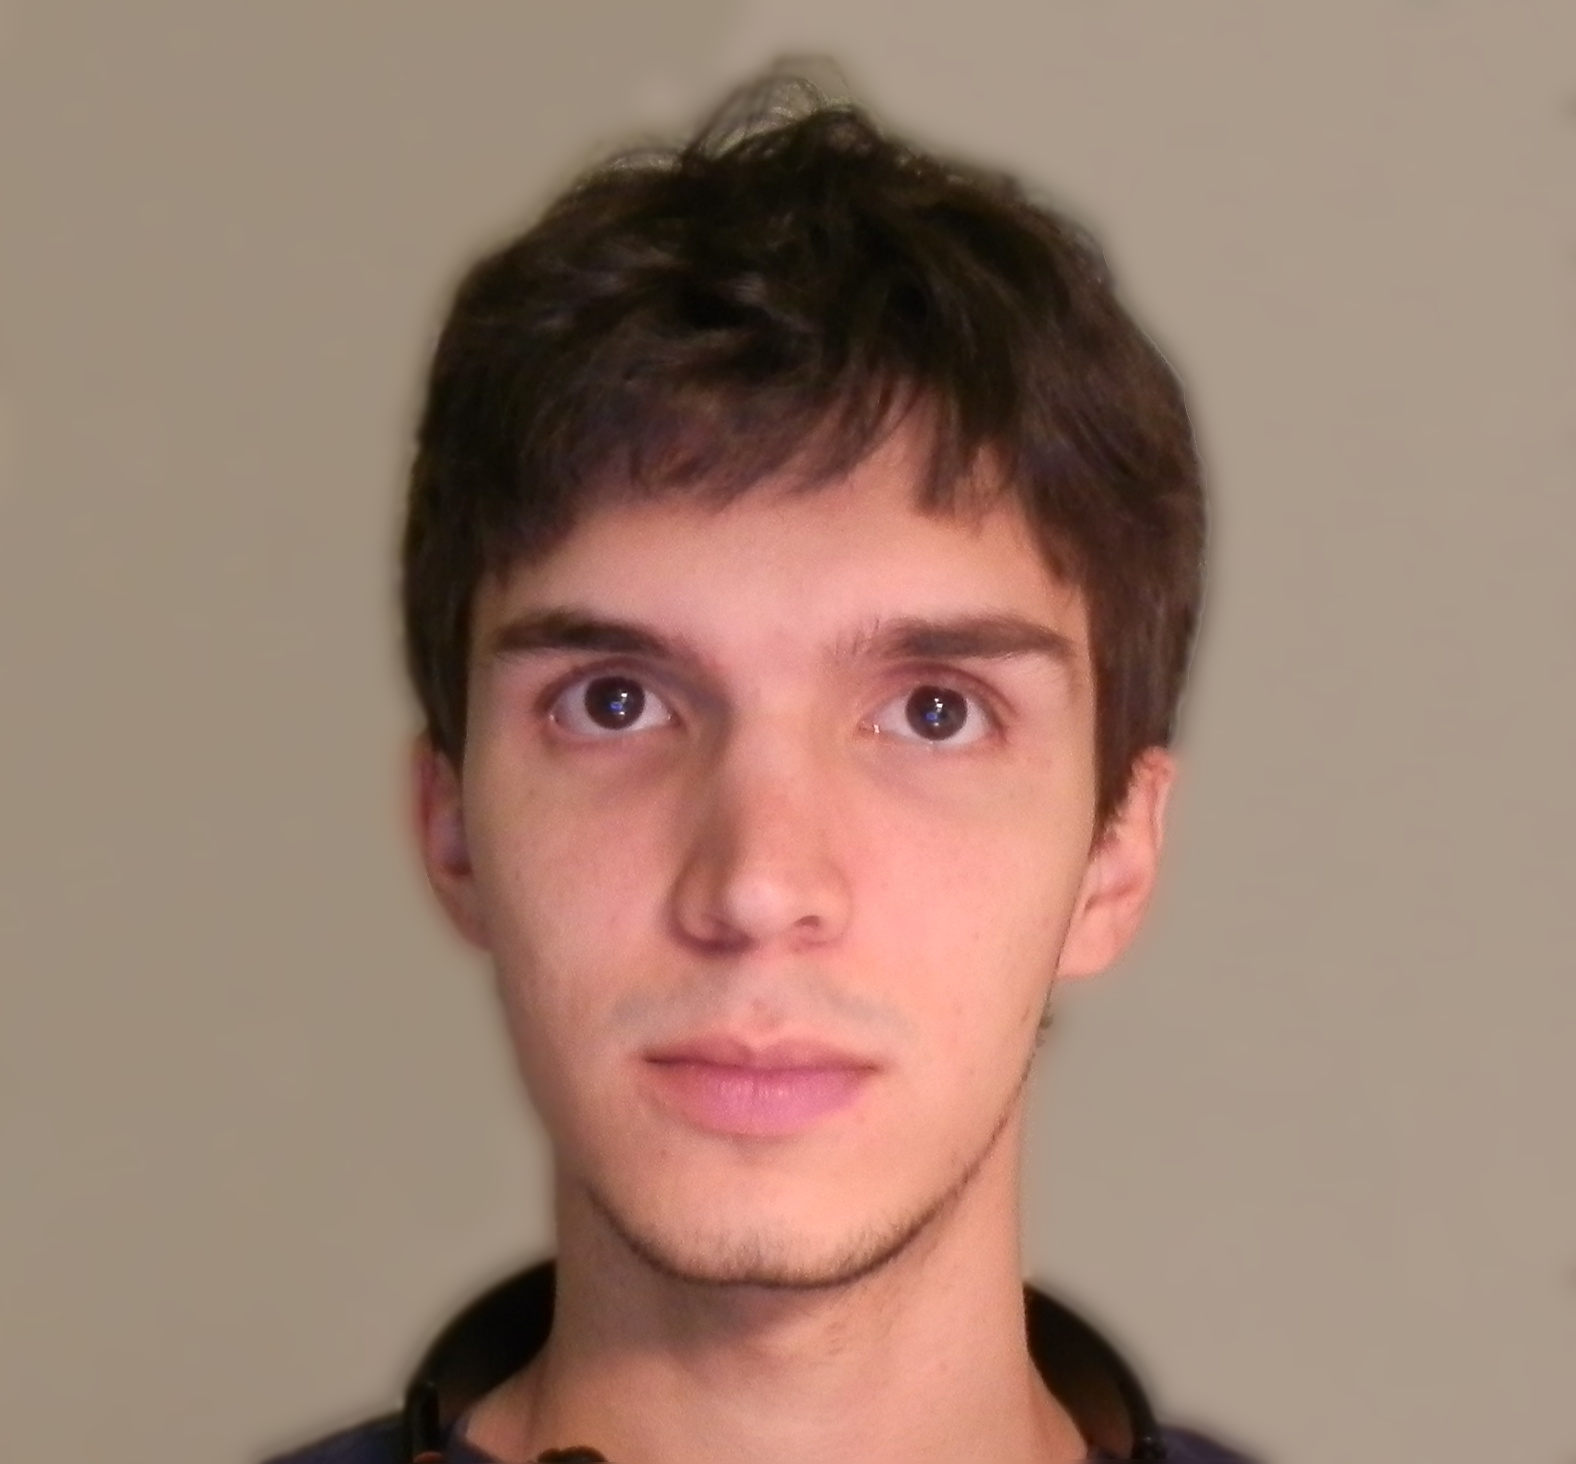
\includegraphics[width=1in,height=1.25in,clip,keepaspectratio]{apereira}}]{Andre Hahn Pereira} is currently pursuing his B.Sc degree in ECE at the University of S\~{a}o Paulo. He was an exchange student at the University of Toronto from September 2012 until August 2013.
\end{IEEEbiography}

\begin{IEEEbiography}[{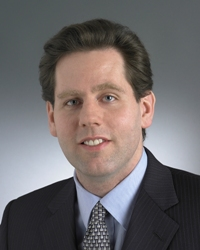
\includegraphics[width=1in,height=1.25in,clip,keepaspectratio]{vbetz}}]{Vaughn Betz}(S'88--M'91) received the B.Sc(EE) from the University of Manitoba in 1991, the MS(ECE) from the University of Illinois at Urbana-Champaign in 1993, and the PhD(ECE) from the University of Toronto in 1998.

Dr. Betz co-founded Right Track CAD, which was acquired by Altera in 2000. He was at Altera from 2000 to 2011, ultimately as Senior Director of Software Engineering. He is now an Associate Professor at the University of Toronto and researchs FPGA architecture, CAD and FPGA-based computation.
\end{IEEEbiography}

% ----------------------------------


\section*{Differences from Previous Work}
This work has not been previously published. It builds upon an earlier conference publication ``CAD and Routing Architecture for Interposer-Based Multi-FPGA Systems,'' A. Hahn Pereira and V. Betz, \textit{ACM Int. Symposium on FPGAs}, 2014, pp. 75 - 84, but greatly improves on and extends this earlier work.  Approximately 75\% of the material in this paper is entirely new methods and new results that are not in the conference paper; the remaining 25\% of the material (chiefly the Introduction, Background, some of the Architecture Models and the Placer Optimization subsection of CAD Enhancements) have been updated since the conference paper but cover the same basic material as the conference paper. In detail, new material includes:

\begin{itemize}
\item Partitioning is now included in the CAD flow. We investigate multiple ways to formulate the partitioning problem for interposer-based FPGAs and compare the results to CAD flows without partitioning. All of Section V of the paper (4 pages) is completely new material vs. the conference paper.

\item Section III, Architecture Models has been expanded vs. the conference paper, and the method of modeling the architecture in the CAD tools is new.  Section III.D is completely new and Section III.E uses a different method than the conference paper and has been rewritten and expanded.

\item Section IV, CAD enhancements contains mostly new material vs. the conference paper. The router enhancements section (IV.B) is entirely new, while the placement enhancement section (IV.A) is shortened and the effectiveness of the enhancements section (IV.C) is new.

\item All of the architecture results have been re-run with the new CAD flow and architectural enhancements proposed in this paper, so all the results in Section VI are different and markedly better than those of the conference paper; this entire section has been re-written. Sections VI.A and VI.E investigate entirely new architecture questions proposed in this paper; there is no analog to these sections in the earlier conference paper.

\item The Introduction, Background and Conclusions (Section I, II and VII) have been updated to highlight the new results of this paper and to describe recent developments in commercial interposer-based FPGAs at 20 nm.
\end {itemize}



% that's all folks
\end{document}


